% !TEX program = xelatex
% 扩散生成模型的数学原理（教案笔记）—— LaTeX 重排版
\documentclass[a4paper,fontset=none,zihao=5]{ctexart}

% ---------------- 字体 ----------------
\setCJKmainfont{NotoSerifCJKsc-Regular}[BoldFont=NotoSerifCJKsc-Bold, ItalicFont={AR PL KaitiM GB}]
\setCJKsansfont{NotoSansCJKsc-Regular}[BoldFont=NotoSansCJKsc-Bold]
\setCJKmonofont{NotoSansMonoCJKsc-Regular}
\setCJKfamilyfont{kai}{AR PL KaitiM GB}
\providecommand{\kaishu}{\CJKfamily{kai}}

% ---------------- 宏包 ----------------
\usepackage[margin=1.8cm,top=2.0cm,bottom=2.0cm]{geometry}
\usepackage{amsmath,amssymb,amsthm,mathtools,bm}
\usepackage{graphicx}
\usepackage{float}
\usepackage{caption}
\usepackage{booktabs}
\usepackage{enumitem}
\usepackage{xcolor}
\usepackage[most]{tcolorbox}
\usepackage{algorithm}
\usepackage{algpseudocode}
\usepackage{fancyhdr}
\usepackage[hidelinks,unicode]{hyperref}

\definecolor{ctitle}{HTML}{1E3A8A}
\definecolor{chead}{HTML}{1E40AF}
\definecolor{csub}{HTML}{334155}
\definecolor{cbox}{HTML}{EFF6FF}
\definecolor{cboxb}{HTML}{93C5FD}
\definecolor{cnote}{HTML}{9A3412}
\definecolor{cnotebg}{HTML}{FFF7ED}
\definecolor{cmuted}{HTML}{64748B}

\hypersetup{
  pdftitle={扩散生成模型的数学原理（教案笔记）},
  pdfauthor={Grok Bot 教学笔记},
  pdfsubject={DDPM / Score-based / Denoising Diffusion},
}

% 标题样式
\ctexset{
  section = {format=\Large\sffamily\bfseries\color{chead}, name={,}, number=\chinese{section}、, aftername={}, beforeskip=1.2em, afterskip=0.7em},
  subsection = {format=\large\sffamily\bfseries\color{csub}, beforeskip=0.9em, afterskip=0.5em},
}

% 页眉页脚
\pagestyle{fancy}
\fancyhf{}
\renewcommand{\headrulewidth}{0.4pt}
\renewcommand{\headrule}{\color{black!15}\hrule height\headrulewidth}
\fancyfoot[C]{\footnotesize\color{cmuted}扩散模型数学原理教案\quad·\quad 第 \thepage{} 页}
\fancypagestyle{plain}{\fancyhf{}\renewcommand{\headrulewidth}{0pt}%
  \fancyfoot[C]{\footnotesize\color{cmuted}扩散模型数学原理教案\quad·\quad 第 \thepage{} 页}}

% 图、算法
\captionsetup{font={small,color=cmuted},labelsep=quad}
\captionsetup[figure]{name=图}
\floatname{algorithm}{算法}
\renewcommand{\algorithmicrequire}{\textbf{输入：}}
\renewcommand{\algorithmicensure}{\textbf{输出：}}
\algrenewcommand\algorithmicrepeat{\textbf{repeat}}
\algrenewcommand\algorithmicuntil{\textbf{until}}

% 公式编号按节
\numberwithin{equation}{section}

% 盒子
\newtcolorbox{notebox}[1][]{enhanced,colback=cnotebg,colframe=cnote!45,boxrule=0.5pt,arc=2pt,
  left=6pt,right=6pt,top=4pt,bottom=4pt,fontupper=\small\color{cnote},#1}
\newtcolorbox{keybox}[1][]{enhanced,colback=cbox,colframe=cboxb,boxrule=0.6pt,arc=2pt,
  left=6pt,right=6pt,top=2pt,bottom=2pt,#1}

\definecolor{cwhy}{HTML}{047857}
\definecolor{cwhybg}{HTML}{ECFDF5}
\newtcolorbox{whybox}[1][]{enhanced,breakable,colback=cwhybg,colframe=cwhy!55,boxrule=0.5pt,arc=2pt,
  left=6pt,right=6pt,top=3pt,bottom=4pt,fontupper=\small,
  title={\sffamily\bfseries 为什么这样做？},coltitle=cwhy,colbacktitle=cwhybg,
  attach title to upper={\quad},#1}

% ---------------- 记号 ----------------
\newcommand{\x}{\mathbf{x}}
\newcommand{\I}{\mathbf{I}}
\newcommand{\N}{\mathcal{N}}
\newcommand{\abar}{\bar{\alpha}}
\newcommand{\eps}{\boldsymbol{\epsilon}}
\newcommand{\epst}{\boldsymbol{\epsilon}_\theta}
\newcommand{\mut}{\tilde{\boldsymbol{\mu}}}
\newcommand{\mutheta}{\boldsymbol{\mu}_\theta}
\newcommand{\btil}{\tilde{\beta}}
\newcommand{\E}{\mathbb{E}}
\newcommand{\KL}[2]{D_{\mathrm{KL}}\!\left(#1\,\middle\|\,#2\right)}
\newcommand{\Lsimple}{L_{\mathrm{simple}}}
\newcommand{\LVLB}{L_{\mathrm{VLB}}}

\setlength{\parskip}{0.3em}
\linespread{1.25}

\begin{document}

% ======================== 封面 ========================
\thispagestyle{plain}
\begin{center}
  \vspace*{1.2cm}
  {\sffamily\bfseries\fontsize{24}{32}\selectfont\color{ctitle} 扩散生成模型的数学原理\par}
  \vspace{0.6em}
  {\large\color{csub} DDPM\enspace·\enspace 噪声预测\enspace·\enspace Score Matching\enspace·\enspace SDE 直觉桥接\par}
  \vspace{0.5em}
  {\color{chead}\rule{0.6\textwidth}{1.5pt}\par}
  \vspace{0.5em}
  {\color{csub} 教案 / 自学笔记（含推导与插图）\par}
  {\color{csub} 面向已熟悉基础概率与深度学习的读者\par}
\end{center}
\vspace{0.8cm}

\subsection*{学习目标}
\begin{enumerate}[leftmargin=2.2em,itemsep=2pt]
  \item 用直觉理解前向加噪与反向去噪如何构成生成模型；
  \item 掌握闭式前向采样公式 $q(\x_t\mid\x_0)$，以及 $\beta_t$ / $\abar_t$ 日程（schedule）的含义；
  \item 理解反向过程的高斯参数化，以及为何常用 $\epst$ 预测噪声；
  \item 理清从变分下界（ELBO）到简化 MSE 训练目标的推导主线；
  \item 能写出（伪代码级）DDPM 采样步骤，并与 score / SDE 观点建立直觉联系。
\end{enumerate}

\vspace{0.4cm}
\noindent\textbf{主要参考}（真实文献，便于对照精读）：
\begin{enumerate}[label={[\arabic*]},leftmargin=2.2em,itemsep=1pt,font=\small]\small
  \item J. Ho, A. Jain, P. Abbeel. \emph{Denoising Diffusion Probabilistic Models}. NeurIPS 2020.
  \item Y. Song, S. Ermon. \emph{Generative Modeling by Estimating Gradients of the Data Distribution}. NeurIPS 2019.
  \item Y. Song, J. Sohl-Dickstein, D. P. Kingma, A. Kumar, S. Ermon, B. Poole. \emph{Score-Based Generative Modeling through Stochastic Differential Equations}. ICLR 2021.
  \item J. Sohl-Dickstein, E. Weiss, N. Maheswaranathan, S. Ganguli. \emph{Deep Unsupervised Learning using Nonequilibrium Thermodynamics}. ICML 2015.
\end{enumerate}

\vspace{0.4cm}
\begin{notebox}
\textbf{记号约定：}$\x_0$ 为干净数据；$\x_t$ 为时刻 $t$ 的带噪样本；$\eps\sim\N(\mathbf{0},\I)$；
$\beta_t$ 为前向噪声日程；$\alpha_t = 1-\beta_t$；$\abar_t=\prod_{s=1}^{t}\alpha_s$（约定 $\abar_0=1$）；
$\epst(\x_t,t)$ 为噪声预测网络；$\mut_t$、$\btil_t$ 分别为（给定 $\x_0$ 时）真实后验的均值与方差。
\end{notebox}

\newpage
% ======================== 一 ========================
\section{直觉图：从清晰图像到噪声，再反向生成}

扩散生成模型（Diffusion Generative Models）的核心思想非常朴素：
先把数据分布通过一条预先设计好的「加噪」马尔可夫链，逐步破坏成近似标准正态；
再学习一条「去噪」马尔可夫链，从纯噪声一步步还原出接近真实数据的样本。
训练时我们只学反向过程的参数 $\theta$；采样时从 $\x_T\sim\N(\mathbf{0},\I)$ 出发迭代去噪得到 $\x_0$。

可以把前向过程想成「把一幅清晰照片慢慢糊成雪花屏」——这是固定的、不需要学习的；
反向过程则是「从雪花屏里一点点恢复出一张新照片」——这才是网络要学的本领。
关键技巧在于：前向加噪有闭式公式，因此训练时不必真的走完所有逐步加噪，
可以直接一次采样任意时刻的 $\x_t$。

\begin{whybox}
\textbf{为什么要分成很多小步，而不是一步从噪声变成数据？}「噪声 $\to$ 数据」的整体映射极其复杂（GAN、VAE 正是试图一步学会它，因此训练困难或样本模糊）。
把它拆成 $T$ 个小步后，每一步只需去掉一点点噪声，这个局部任务简单得多，并且小步下反向转移近似为高斯（见 3.2 节），可以用简单的高斯模型加上一个去噪网络来表示。
代价是采样需要多步迭代。
\end{whybox}

\setcounter{figure}{-1}% 与图片内嵌标题编号保持一致
\begin{figure}[H]
  \centering
  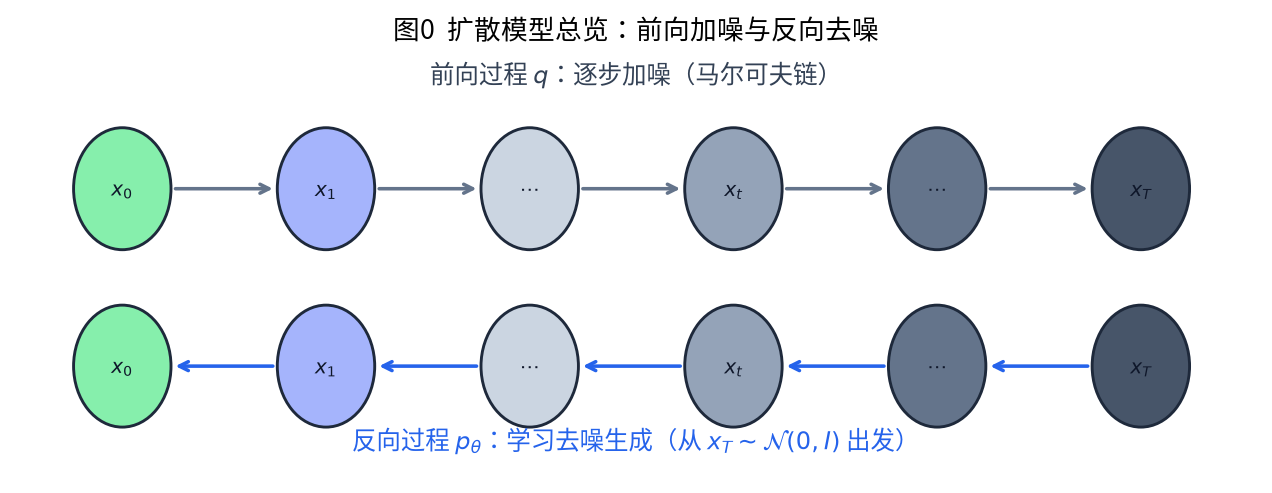
\includegraphics[width=0.86\textwidth]{figures/fig0_overview_pipeline.png}
  \caption{前向加噪（上）与反向去噪生成（下）总览}
  \label{fig:overview}
\end{figure}

\noindent 图~\ref{fig:overview} 用颜色深浅示意噪声含量：左侧 $\x_0$ 偏「干净」，右侧 $\x_T$ 接近各向同性高斯。
生成时箭头反向：从右端噪声出发，沿 $p_\theta$ 逐步走到左端数据流形附近。

\setcounter{figure}{3}% 与图片内嵌标题编号保持一致
\begin{figure}[H]
  \centering
  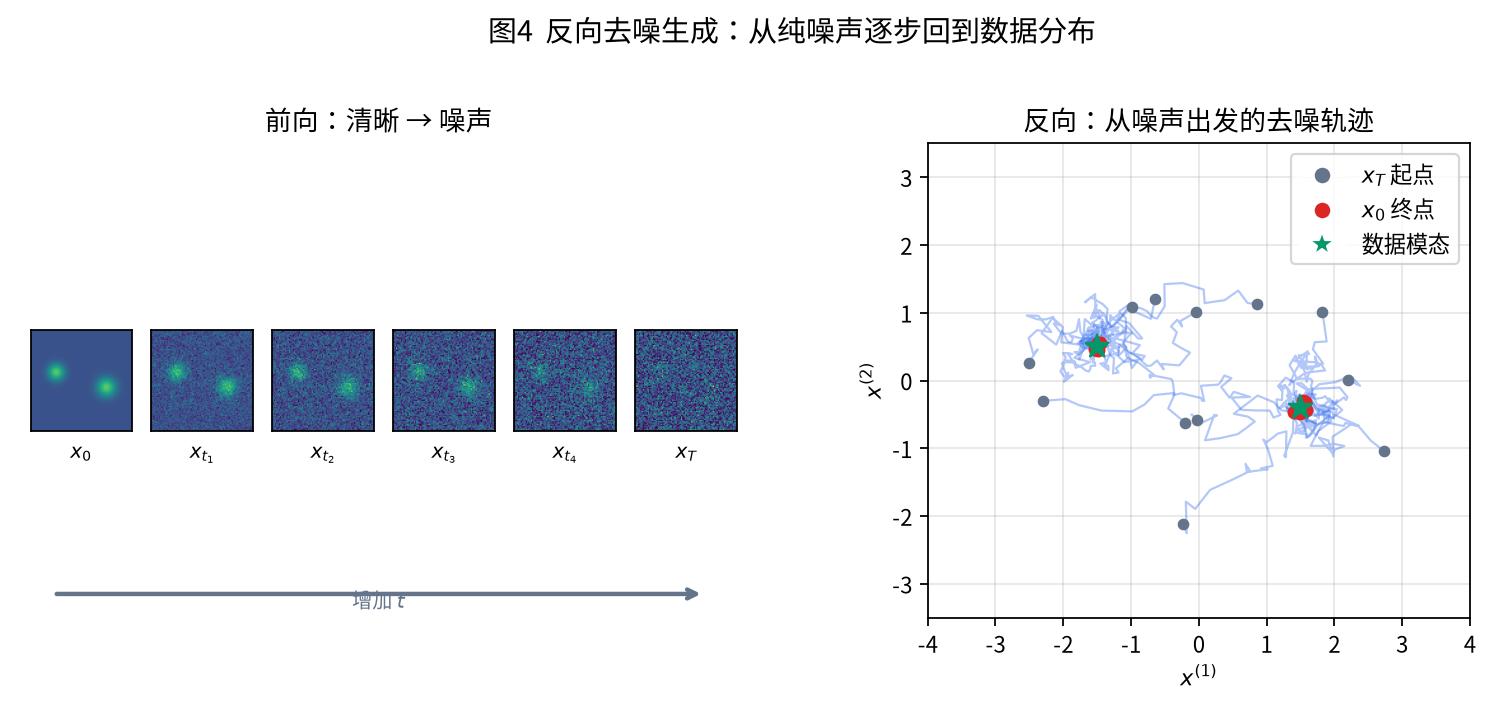
\includegraphics[width=0.86\textwidth]{figures/fig4_reverse_trajectory.png}
  \caption{左：前向破坏结构；右：多条反向轨迹汇聚到数据模态}
  \label{fig:traj}
\end{figure}

\newpage
% ======================== 二 ========================
\section{前向过程：马尔可夫链与闭式 \texorpdfstring{$q(\x_t\mid\x_0)$}{q(x\_t|x\_0)}}

\subsection{逐步加噪定义}
给定数据 $\x_0\sim q(\x_0)$，前向过程定义为固定的马尔可夫链：每一步对当前状态加入少量高斯噪声。
\begin{keybox}
\begin{align}
  q(\x_t\mid\x_{t-1}) &= \N\!\left(\x_t;\ \sqrt{1-\beta_t}\,\x_{t-1},\ \beta_t\I\right), \label{eq:fwd-step}\\
  q(\x_{1:T}\mid\x_0) &= \prod_{t=1}^{T} q(\x_t\mid\x_{t-1}). \label{eq:fwd-joint}
\end{align}
\end{keybox}
其中 $\beta_t\in(0,1)$ 是预先选定的方差日程（variance schedule）。$\beta_t$ 很小时，每一步只轻微扰动；
当 $T$ 足够大、使得 $\abar_T=\prod_{t=1}^T(1-\beta_t)\approx 0$ 时，$\x_T$ 的分布会接近 $\N(\mathbf{0},\I)$，几乎与 $\x_0$ 无关。

\begin{whybox}
\textbf{为什么均值要乘 $\sqrt{1-\beta_t}$，而不是直接 $\x_t=\x_{t-1}+\sqrt{\beta_t}\,\eps_t$？}
设数据已归一化为单位方差，$\mathrm{Var}(\x_{t-1})=1$。按 \eqref{eq:fwd-step}，
\[
  \mathrm{Var}(\x_t)=(1-\beta_t)\,\mathrm{Var}(\x_{t-1})+\beta_t=(1-\beta_t)+\beta_t=1,
\]
方差在每一步都\emph{保持不变}（variance preserving，VP）：信号被缩小的部分正好由噪声补上。
若不缩放，方差会累加为 $1+\sum_t\beta_t$ 而不断增大（这是 VE 型设计），终点就不是固定的 $\N(\mathbf{0},\I)$。
VP 设计的好处：(i) 终点分布确定为 $\N(\mathbf{0},\I)$，采样起点与数据无关；(ii) 网络在所有 $t$ 上看到的输入尺度一致，便于训练。
\end{whybox}

\subsection{记号：\texorpdfstring{$\alpha_t$ 与 $\abar_t$}{alpha\_t 与 alpha-bar\_t}}
\begin{equation}
  \alpha_t \coloneqq 1-\beta_t, \qquad \abar_t \coloneqq \prod_{s=1}^{t}\alpha_s .
  \label{eq:alphabar}
\end{equation}
$\abar_t$ 刻画了「到时刻 $t$ 为止，原始信号还剩多少比例」（信号方差比例）。$\abar_t$ 随 $t$ 单调递减：
$t$ 接近 $0$ 时 $\abar_t\approx 1$（几乎全是信号），$t\to T$ 时 $\abar_t\to 0$（几乎全是噪声）。

\subsection{闭式边缘分布（关键公式）}
利用高斯分布的再生性（独立高斯之和仍为高斯），可以把多步加噪坍缩成一步。令 $\eps\sim\N(\mathbf{0},\I)$，则
\begin{keybox}
\begin{align}
  \x_t &= \sqrt{\abar_t}\,\x_0 + \sqrt{1-\abar_t}\,\eps, \label{eq:closed}\\
  \text{亦即}\quad q(\x_t\mid\x_0) &= \N\!\left(\x_t;\ \sqrt{\abar_t}\,\x_0,\ (1-\abar_t)\I\right). \label{eq:closed-dist}
\end{align}
\end{keybox}
\textbf{推导要点（归纳法）。}由 \eqref{eq:fwd-step}，$\x_1=\sqrt{\alpha_1}\,\x_0+\sqrt{1-\alpha_1}\,\eps_1$，结论对 $t=1$ 成立。
假设 $\x_{t-1}=\sqrt{\abar_{t-1}}\,\x_0+\sqrt{1-\abar_{t-1}}\,\tilde{\eps}$，代入 $\x_t=\sqrt{\alpha_t}\,\x_{t-1}+\sqrt{1-\alpha_t}\,\eps_t$：
\begin{equation}
  \x_t = \sqrt{\alpha_t\abar_{t-1}}\,\x_0
        + \underbrace{\sqrt{\alpha_t(1-\abar_{t-1})}\,\tilde{\eps} + \sqrt{1-\alpha_t}\,\eps_t}_{\sim\,\N\left(\mathbf{0},\ [\alpha_t(1-\abar_{t-1}) + (1-\alpha_t)]\I\right)} .
\end{equation}
合并的噪声方差为 $\alpha_t(1-\abar_{t-1})+(1-\alpha_t)=1-\alpha_t\abar_{t-1}=1-\abar_t$，且 $\alpha_t\abar_{t-1}=\abar_t$，即得 \eqref{eq:closed}。（「两个独立高斯噪声合并为一个」的引理与逐行推导见 \ref{sec:reparam} 节。）
这一闭式使训练时可对任意 $t$ 直接构造 $\x_t$，无需模拟整条链。

\begin{whybox}
\textbf{为什么闭式 $q(\x_t\mid\x_0)$ 对训练如此重要？}训练目标是对 $t=1,\dots,T$ 的各项求和（第四节）。
有了闭式，就可以\emph{随机抽一个} $t\sim\mathrm{Uniform}\{1,\dots,T\}$，一步得到 $\x_t$，用这一项的梯度作为整体求和的\emph{无偏}估计
（$\sum_t L_t=T\cdot\E_t[L_t]$）。每个训练样本的代价是 $O(1)$ 次网络前向，而不是 $O(T)$；
同一批次中不同样本取不同 $t$，网络同时学会所有噪声水平。
\end{whybox}

\subsection{重参数化技巧（reparameterization trick）详解}
\label{sec:reparam}
上面的闭式 \eqref{eq:closed} 把「$\x_t$ 服从某个高斯」写成了「$\x_t$ 是 $\x_0$ 与一个标准噪声 $\eps$ 的确定性函数」。
这种写法就是\textbf{重参数化技巧}。它在 DDPM 中出现了至少四次（前向一步、闭式推导、训练、采样），下面把它单独讲透。

\paragraph{(1) 它是什么：位置-尺度变换。}任何各向同性高斯都可以由标准高斯经平移、缩放得到：
\begin{keybox}
\begin{equation}
  \mathbf{z}\sim\N(\boldsymbol{\mu},\sigma^2\I)
  \quad\Longleftrightarrow\quad
  \mathbf{z}=\boldsymbol{\mu}+\sigma\,\eps,\qquad \eps\sim\N(\mathbf{0},\I).
  \label{eq:reparam}
\end{equation}
\end{keybox}
\textbf{证明一（矩 + 仿射不变性）。}高斯向量经仿射变换仍是高斯，因此只需核对均值与协方差：
\begin{align}
  \E[\mathbf{z}] &= \boldsymbol{\mu}+\sigma\,\E[\eps]=\boldsymbol{\mu}, \notag\\
  \mathrm{Cov}[\mathbf{z}] &= \E\big[(\mathbf{z}-\boldsymbol{\mu})(\mathbf{z}-\boldsymbol{\mu})^\top\big]
   =\sigma^2\,\E[\eps\eps^\top]=\sigma^2\I. \notag
\end{align}
\textbf{证明二（变量替换）。}$\eps=(\mathbf{z}-\boldsymbol{\mu})/\sigma$，雅可比行列式 $\big|\det\frac{\partial\eps}{\partial\mathbf{z}}\big|=\sigma^{-d}$（$d$ 为维数），故
\begin{equation}
  p_{\mathbf{z}}(\mathbf{z})=p_{\eps}\Big(\frac{\mathbf{z}-\boldsymbol{\mu}}{\sigma}\Big)\,\sigma^{-d}
  =\frac{1}{(2\pi)^{d/2}\sigma^{d}}\exp\!\Big(-\frac{\|\mathbf{z}-\boldsymbol{\mu}\|^2}{2\sigma^2}\Big)=\N(\mathbf{z};\boldsymbol{\mu},\sigma^2\I).
\end{equation}
（一般协方差 $\boldsymbol{\Sigma}=\mathbf{L}\mathbf{L}^\top$ 时写成 $\mathbf{z}=\boldsymbol{\mu}+\mathbf{L}\eps$。）

\begin{whybox}
\textbf{这一改写的本质：把「随机性」和「参数 / 输入」分开。}左边「从 $\N(\boldsymbol{\mu},\sigma^2\I)$ 中抽样」是一个依赖参数的随机操作；
右边的随机性全部集中在\emph{不含任何参数}的 $\eps$ 上，而 $\boldsymbol{\mu},\sigma$ 只通过一个普通的、可微的算术式 $\boldsymbol{\mu}+\sigma\eps$ 进入。
于是：采样变成「先抽固定分布的噪声，再做确定性计算」；而且只要记住所用的 $\eps$，就知道样本是「怎么来的」。
\textbf{为什么系数是 $\sigma$ 而不是 $\sigma^2$？}乘在 $\eps$ 前面的是\emph{标准差}：$\mathrm{Var}(\sigma\eps)=\sigma^2$。
所以方差为 $\beta_t$ 的噪声写成 $\sqrt{\beta_t}\,\eps$，方差为 $1-\abar_t$ 的写成 $\sqrt{1-\abar_t}\,\eps$——公式里那些根号都来源于此。
\end{whybox}

\paragraph{(2) 它为什么重要：来自 VAE 的梯度问题。}
Kingma \& Welling（2014，VAE）与 Rezende et al.（2014）提出这个技巧，是为了计算
$\nabla_\phi\,\E_{\mathbf{z}\sim q_\phi}[f(\mathbf{z})]$——期望所对的分布本身依赖参数 $\phi$，而「抽样」这一步对 $\phi$ 不可微（图~\ref{fig:reparam}(a)）。有两种估计方式：
\begin{align}
  \text{得分函数 / REINFORCE：}\quad
  \nabla_\phi\,\E_{q_\phi}[f(\mathbf{z})]
  &=\int f(\mathbf{z})\,\nabla_\phi q_\phi(\mathbf{z})\,\mathrm{d}\mathbf{z}
   =\E_{q_\phi}\!\big[f(\mathbf{z})\,\nabla_\phi\log q_\phi(\mathbf{z})\big], \label{eq:reinforce}\\
  \text{重参数化 / 路径导数：}\quad
  \nabla_\phi\,\E_{q_\phi}[f(\mathbf{z})]
  &=\nabla_\phi\,\E_{\eps}\big[f(\boldsymbol{\mu}_\phi+\sigma_\phi\eps)\big]
   =\E_{\eps}\Big[\nabla_{\mathbf{z}}f(\mathbf{z})^\top\Big(\frac{\partial\boldsymbol{\mu}_\phi}{\partial\phi}+\eps\,\frac{\partial\sigma_\phi}{\partial\phi}\Big)\Big]. \label{eq:pathwise}
\end{align}
\eqref{eq:reinforce} 用到恒等式 $\nabla_\phi q_\phi=q_\phi\nabla_\phi\log q_\phi$；
\eqref{eq:pathwise} 中 $\eps$ 的分布与 $\phi$ 无关，梯度可直接移进期望（图~\ref{fig:reparam}(b)），其中 $\mathbf{z}=\boldsymbol{\mu}_\phi+\sigma_\phi\eps$。

\textbf{一个可以手算的例子。}$z\sim\N(\mu,1)$，$f(z)=z^2$，对 $\mu$ 求导。真值：$\E[z^2]=\mu^2+1$，梯度 $=2\mu$。
\begin{itemize}[leftmargin=1.6em,itemsep=1pt]
  \item 路径导数：单样本估计 $2z=2(\mu+\epsilon)$，均值 $2\mu$，方差 $\mathrm{Var}(2\epsilon)=4$。
  \item REINFORCE：$\nabla_\mu\log q=z-\mu=\epsilon$，单样本估计 $(\mu+\epsilon)^2\epsilon$，均值 $\E[\mu^2\epsilon+2\mu\epsilon^2+\epsilon^3]=2\mu$；
        利用 $\E[\epsilon^2]=1,\E[\epsilon^4]=3,\E[\epsilon^6]=15$，可得二阶矩 $\E[(\mu+\epsilon)^4\epsilon^2]=\mu^4+18\mu^2+15$，
        方差 $=\mu^4+14\mu^2+15$（$\mu=0$ 时为 $15$，$\mu=2$ 时为 $87$）。
\end{itemize}
两者都无偏，但路径导数利用了 $f$ 的梯度信息，方差通常小得多；REINFORCE 只用到 $f$ 的取值，方差随 $|f|$ 增大，需要基线（baseline）等降方差技巧。

\begin{whybox}
\textbf{为什么在 VAE 里非用不可？}编码器输出 $\boldsymbol{\mu}_\phi(\x),\sigma_\phi(\x)$，解码器的重构误差要对编码器参数 $\phi$ 求导，
而中间隔着一个「采样 $\mathbf{z}$」。重参数化把这个采样节点换成可微的 $\boldsymbol{\mu}_\phi+\sigma_\phi\eps$，反向传播即可一路走通。
这要求分布属于\emph{位置-尺度族}（如高斯、拉普拉斯、逻辑斯谛）或至少有可微的采样变换；离散分布（如类别分布）不能直接这样做（需 Gumbel-Softmax 等松弛）。
\end{whybox}

\setcounter{figure}{5}% 新增图6
\begin{figure}[H]
  \centering
  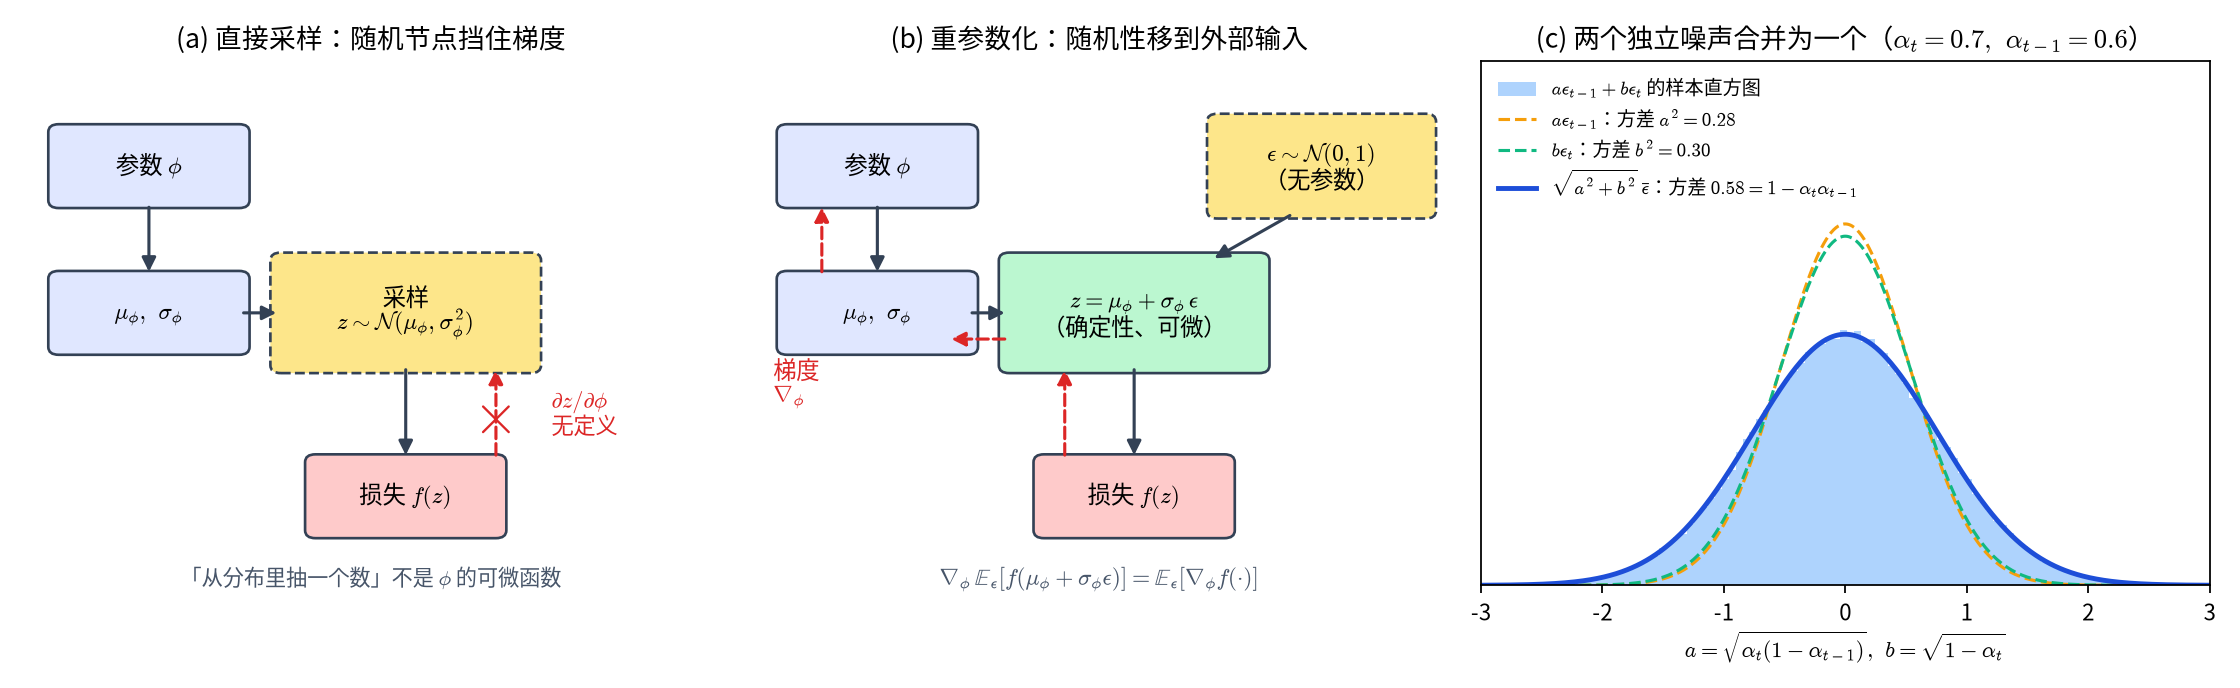
\includegraphics[width=\textwidth]{figures/fig6_reparameterization.png}
  \caption{重参数化技巧。(a) 直接从 $\N(\mu_\phi,\sigma_\phi^2)$ 采样：采样节点对 $\phi$ 不可微，梯度传不回去；
  (b) 写成 $z=\mu_\phi+\sigma_\phi\epsilon$：随机性来自无参数的外部输入 $\epsilon$，梯度沿确定性路径回传；
  (c) 两个独立高斯噪声之和仍是高斯，方差相加：$a^2+b^2=1-\alpha_t\alpha_{t-1}$（直方图为 $2\times10^5$ 个样本）。}
  \label{fig:reparam}
\end{figure}

\paragraph{(3a) 扩散中的用法一：前向单步。}定义 \eqref{eq:fwd-step} 用重参数化写就是
\begin{equation}
  \x_t=\sqrt{\alpha_t}\,\x_{t-1}+\sqrt{\beta_t}\,\eps_t,\qquad \eps_t\sim\N(\mathbf{0},\I),\ \ \eps_1,\dots,\eps_T\ \text{相互独立且与}\ \x_0\ \text{独立}.
  \label{eq:fwd-reparam}
\end{equation}

\paragraph{(3b) 用法二：推导闭式——合并独立高斯噪声（DDPM 里最常说的「重参数化技巧」）。}
\textbf{引理。}若 $\eps_1,\eps_2\sim\N(\mathbf{0},\I)$ 独立，则 $a\eps_1+b\eps_2\sim\N\big(\mathbf{0},(a^2+b^2)\I\big)$，
即可写成 $\sqrt{a^2+b^2}\,\bar{\eps}$，$\bar{\eps}\sim\N(\mathbf{0},\I)$。
\emph{证明：}独立随机变量之和的特征函数是乘积，
$\E[e^{i\mathbf{u}^\top(a\eps_1+b\eps_2)}]=e^{-a^2\|\mathbf{u}\|^2/2}\,e^{-b^2\|\mathbf{u}\|^2/2}=e^{-(a^2+b^2)\|\mathbf{u}\|^2/2}$，正是 $\N(\mathbf{0},(a^2+b^2)\I)$ 的特征函数。
（直观：独立 $\Rightarrow$ 方差相加，均值仍为 $\mathbf{0}$。注意相加的是\emph{方差} $a^2,b^2$，而不是系数 $a,b$。）

\textbf{两步合并，逐行计算。}从 $\x_{t-2}$ 出发连续用两次 \eqref{eq:fwd-reparam}：
\begin{align}
  \x_{t-1} &= \sqrt{\alpha_{t-1}}\,\x_{t-2}+\sqrt{1-\alpha_{t-1}}\,\eps_{t-1}, \notag\\
  \x_t &= \sqrt{\alpha_t}\,\x_{t-1}+\sqrt{1-\alpha_t}\,\eps_t \notag\\
       &= \sqrt{\alpha_t}\Big(\sqrt{\alpha_{t-1}}\,\x_{t-2}+\sqrt{1-\alpha_{t-1}}\,\eps_{t-1}\Big)+\sqrt{1-\alpha_t}\,\eps_t \notag\\
       &= \sqrt{\alpha_t\alpha_{t-1}}\,\x_{t-2}
          +\underbrace{\sqrt{\alpha_t(1-\alpha_{t-1})}}_{a}\,\eps_{t-1}
          +\underbrace{\sqrt{1-\alpha_t}}_{b}\,\eps_t . \label{eq:two-step}
\end{align}
两项噪声独立，由引理，方差相加：
\begin{equation}
  a^2+b^2=\alpha_t(1-\alpha_{t-1})+(1-\alpha_t)=\alpha_t-\alpha_t\alpha_{t-1}+1-\alpha_t=1-\alpha_t\alpha_{t-1},
\end{equation}
所以
\begin{equation}
  \x_t=\sqrt{\alpha_t\alpha_{t-1}}\,\x_{t-2}+\sqrt{1-\alpha_t\alpha_{t-1}}\;\bar{\eps}_{t-2},\qquad\bar{\eps}_{t-2}\sim\N(\mathbf{0},\I).
\end{equation}
\textbf{模式：}信号系数的平方 $\alpha_t\alpha_{t-1}$ 与噪声方差 $1-\alpha_t\alpha_{t-1}$ 之和恒为 $1$。
继续往回合并（即 2.3 节的归纳法）得到 $\x_t=\sqrt{\abar_t}\,\x_0+\sqrt{1-\abar_t}\,\eps$。

\textbf{不用归纳、一次性展开的验证。}把 \eqref{eq:fwd-reparam} 从 $s=t$ 一路代回到 $s=1$：
\begin{equation}
  \x_t=\sqrt{\abar_t}\,\x_0+\sum_{s=1}^{t}\sqrt{\frac{\abar_t}{\abar_s}\,\beta_s}\;\eps_s ,
\end{equation}
（$\eps_s$ 前的系数 $=\sqrt{\beta_s}\times\sqrt{\alpha_{s+1}\cdots\alpha_t}$），噪声总方差为望远镜求和：
\begin{equation}
  \sum_{s=1}^{t}\frac{\abar_t}{\abar_s}(1-\alpha_s)
  =\sum_{s=1}^{t}\Big(\frac{\abar_t}{\abar_s}-\frac{\abar_t}{\abar_{s-1}}\Big)
  =\frac{\abar_t}{\abar_t}-\frac{\abar_t}{\abar_0}=1-\abar_t ,
\end{equation}
（用到 $\abar_s=\alpha_s\abar_{s-1}$ 与 $\abar_0=1$），与 \eqref{eq:closed} 一致。

\paragraph{(3c) 用法三：训练。}算法~\ref{alg:train} 中每次抽 $t,\ \eps$，一步构造 $\x_t=\sqrt{\abar_t}\,\x_0+\sqrt{1-\abar_t}\,\eps$，
网络输入是 $(\x_0,\eps)$ 的确定性可微函数，损失为 $\|\eps-\epst(\x_t,t)\|^2$。注意：
\begin{equation}
  \nabla_\theta\,\E_{t,\x_0,\eps}\Big[\big\|\eps-\epst\big(\sqrt{\abar_t}\,\x_0+\sqrt{1-\abar_t}\,\eps,\ t\big)\big\|^2\Big]
  =\E_{t,\x_0,\eps}\Big[\nabla_\theta\big\|\eps-\epst(\cdots)\big\|^2\Big].
\end{equation}
这里求导只针对网络参数 $\theta$；前向过程\emph{没有}可学参数，期望所对的分布本来就与 $\theta$ 无关。所以在标准 DDPM 中，
重参数化的作用\emph{不是}像 VAE 那样「让梯度穿过采样节点」，而是：
\begin{enumerate}[leftmargin=1.8em,itemsep=1pt,label=(\roman*)]
  \item \textbf{$O(1)$ 采样 $\x_t$：}任意 $t$ 一步到位，无需模拟 $t$ 步（2.3 节为什么框）；
  \item \textbf{给出回归标签：}构造 $\x_t$ 所用的那个 $\eps$ 被记录下来，正好作为监督学习的目标——「已知答案的去噪练习题」；
  \item \textbf{在 $\x_0$ 与 $\eps$ 之间换算：}给定 $\x_t$，由 $\x_0=(\x_t-\sqrt{1-\abar_t}\,\eps)/\sqrt{\abar_t}$ 可以把 $\mut_t$ 改写成 $\eps$ 形式（3.5 节式 \eqref{eq:mut-eps}），
        也是 4.3 节把 KL 化为噪声 MSE 的关键一步。
\end{enumerate}
（只有当前向过程本身含可学参数时——例如 Variational Diffusion Models（Kingma et al., NeurIPS 2021）学习噪声日程——梯度才需要像 VAE 那样穿过 $\x_t$ 的重参数化路径。）

\paragraph{(3d) 用法四：采样。}算法~\ref{alg:sample} 中的 $\x_{t-1}=\mutheta(\x_t,t)+\sigma_t\mathbf{z}$，$\mathbf{z}\sim\N(\mathbf{0},\I)$，
就是对反向高斯 $p_\theta(\x_{t-1}\mid\x_t)=\N(\mutheta,\sigma_t^2\I)$ 的重参数化采样：先抽无参数噪声 $\mathbf{z}$，再做确定性的平移与缩放。

\begin{notebox}
\textbf{澄清：DDPM 文献里的「重参数化」有两层意思，别混淆。}
\begin{center}
\small
\begin{tabular}{p{0.15\textwidth}p{0.38\textwidth}p{0.36\textwidth}}
  \toprule
  & \textbf{A. 采样重参数化} & \textbf{B. 模型参数化（parameterization）} \\
  \midrule
  是什么 & 把随机变量写成「确定性函数 $+$ 无参数噪声」：$\mathbf{z}=\boldsymbol{\mu}+\sigma\eps$ & 选择网络\emph{输出什么量}：$\eps$、$\x_0$ 还是 $\mut$（或 $\mathbf{v}$、得分） \\
  出现位置 & 前向单步、闭式合并、构造 $\x_t$、祖先采样 & 3.5–3.6 节的 $\mutheta$ 写法 \eqref{eq:mu-eps}；4.3 节 $\Lsimple$ \\
  改变了什么 & 计算方式；分布不变 & 网络的学习目标与优化难度；模型族不变（可互相换算） \\
  \bottomrule
\end{tabular}
\end{center}
Ho et al.（2020）说「$\eps$-prediction parameterization」指的是 B；但 B 之所以可行，正是借助了 A 给出的关系 $\x_t=\x_t(\x_0,\eps)$。
\end{notebox}

\begin{notebox}
\textbf{常见坑。}
\begin{enumerate}[leftmargin=1.6em,itemsep=1pt]
  \item \textbf{每一步的噪声必须是新抽的、相互独立的。}$\eps_1,\dots,\eps_T$ 若重复使用同一个，噪声就不再独立，引理不成立（方差变成 $(a+b)^2$ 而非 $a^2+b^2$）。采样时每步的 $\mathbf{z}$ 也必须重新抽取。
  \item \textbf{合并后的 $\bar{\eps}$ 是一个新变量。}$\bar{\eps}=(a\eps_{t-1}+b\eps_t)/\sqrt{a^2+b^2}$ 与 $\eps_{t-1}$、$\eps_t$ 都相关，但不等于其中任何一个。
        闭式 \eqref{eq:closed} 中的 $\eps$ 是「把 $1\dots t$ 步所有噪声合并成的那一个」，训练时直接抽它即可，不必（也不能）还原出各步的 $\eps_s$。
  \item \textbf{系数是标准差，不是方差。}方差为 $\beta_t$ 的噪声写 $\sqrt{\beta_t}\,\eps$；合并时把\emph{系数平方后相加}再开根号。
  \item \textbf{需要位置-尺度族（或可微采样变换）。}高斯天然满足；离散或其他分布不能照搬 $\boldsymbol{\mu}+\sigma\eps$。
  \item \textbf{引理要求独立。}$\x_{t-1}$ 中的噪声只依赖 $\eps_1,\dots,\eps_{t-1}$，与新的 $\eps_t$ 独立，所以每次合并都合法。
\end{enumerate}
\end{notebox}

\subsection{\texorpdfstring{$\beta$}{beta} 日程的直觉}
经典 DDPM 常用线性日程：$\beta_t$ 从 $\beta_1=10^{-4}$ 线性增至 $\beta_T=0.02$（$T=1000$）。
也有 cosine schedule（Nichol \& Dhariwal, 2021）使中间时段信号衰减更平滑。
选择原则：既要让 $\x_T$ 充分接近标准正态，又要避免过早把信号毁掉，导致后期去噪过难。

\setcounter{figure}{0}% 与图片内嵌标题编号保持一致
\begin{figure}[H]
  \centering
  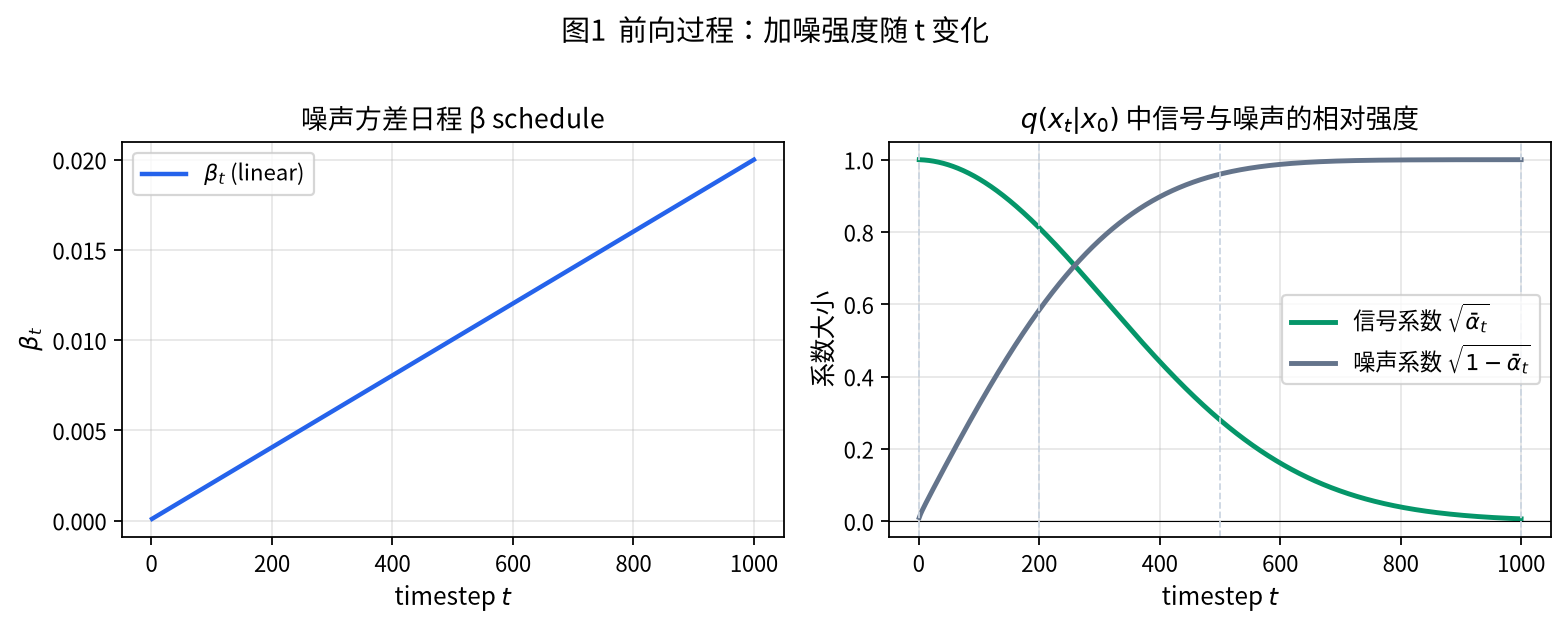
\includegraphics[width=0.86\textwidth]{figures/fig1_forward_schedule.png}
  \caption{左：线性 $\beta_t$；右：$\sqrt{\abar_t}$（信号系数）与 $\sqrt{1-\abar_t}$（噪声系数）随 $t$ 的变化}
  \label{fig:schedule}
\end{figure}

\setcounter{figure}{1}% 与图片内嵌标题编号保持一致
\begin{figure}[H]
  \centering
  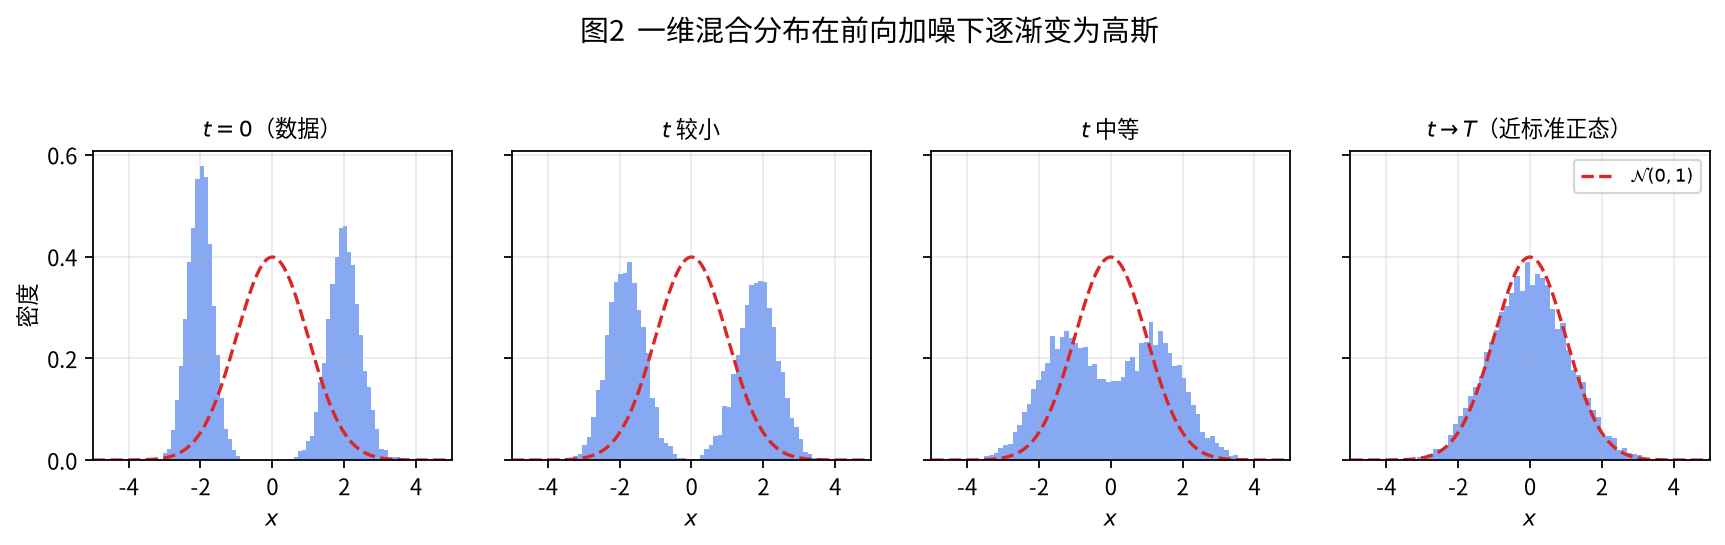
\includegraphics[width=0.86\textwidth]{figures/fig2_1d_gaussianization.png}
  \caption{一维双峰分布在前向加噪下逐渐「高斯化」}
  \label{fig:gauss1d}
\end{figure}

\noindent 图~\ref{fig:gauss1d} 直观说明：无论原始数据多么多峰、复杂，足够强的各向同性高斯噪声会抹平结构，
使分布逼近 $\N(\mathbf{0},\I)$。这也解释了为何可以从「与数据无关」的先验噪声开始生成。

\newpage
% ======================== 三 ========================
\section{反向过程：从贝叶斯公式一步步推导}

本节目标：搞清楚「反向一步」应该长什么样，并把它写成网络可以学习的形式。路线是
\[
  \underbrace{q(\x_{t-1}\mid\x_t)}_{\text{真正想要，但算不出}}
  \;\longrightarrow\;
  \underbrace{q(\x_{t-1}\mid\x_t,\x_0)}_{\text{加条件 $\x_0$ 后可精确计算}}
  \;\longrightarrow\;
  \underbrace{p_\theta(\x_{t-1}\mid\x_t)}_{\text{用网络去逼近}} .
\]

\subsection{真实反向转移为什么算不出来}
由贝叶斯公式，真实的反向转移为
\begin{equation}
  q(\x_{t-1}\mid\x_t) = \frac{q(\x_t\mid\x_{t-1})\,q(\x_{t-1})}{q(\x_t)},
  \qquad
  q(\x_{t-1}) = \int q(\x_{t-1}\mid\x_0)\,q(\x_0)\,\mathrm{d}\x_0 .
  \label{eq:true-rev}
\end{equation}

\begin{whybox}
\textbf{为什么 $q(\x_{t-1}\mid\x_t)$ 不可直接用？}分子里的 $q(\x_{t-1})$、分母里的 $q(\x_t)$ 都是\emph{带噪数据的边缘分布}，
需要对未知的数据分布 $q(\x_0)$ 积分。我们手里只有有限个样本，没有 $q(\x_0)$ 的解析式；
即便用经验分布代替，结果也只是在训练样本之间「插值 / 记忆」，无法泛化出新样本。

\textbf{为什么加上条件 $\x_0$ 就可算？}一旦把 $\x_0$ 当作已知，式中出现的所有分布——
$q(\x_t\mid\x_{t-1})$、$q(\x_{t-1}\mid\x_0)$、$q(\x_t\mid\x_0)$——都是\emph{我们自己设计的}高斯（式 \eqref{eq:fwd-step}、\eqref{eq:closed-dist}），
对未知 $q(\x_0)$ 的依赖消失了。训练时 $\x_0$ 恰好是已知的（就是那张训练图），所以可以用它构造「标准答案」。
\end{whybox}

\subsection{为什么可以把反向一步建模为高斯}
3.4 节将证明：\emph{给定 $\x_0$} 时后验 $q(\x_{t-1}\mid\x_t,\x_0)$ 精确是高斯。但网络 $p_\theta(\x_{t-1}\mid\x_t)$ 看不到 $\x_0$，
它真正要逼近的是\emph{不带 $\x_0$} 的真实反向转移 $q(\x_{t-1}\mid\x_t)$——这是许多高斯按 $q(\x_0\mid\x_t)$ 加权的混合，一般\emph{不是}高斯。
那凭什么还能用一个高斯去建模它？下面分五步说明：答案是「步子足够小」。

\paragraph{第 1 步：从贝叶斯公式出发，一步步写出对数后验。}
记 $q_{t-1}(\cdot)$ 为 $\x_{t-1}$ 的真实边缘分布（未知、一般非高斯，例如多峰），$q_t(\cdot)$ 同理。下面分 5 个小步，从贝叶斯公式走到「平方差」形式。

\textbf{(1a) 贝叶斯公式，并去掉与 $\x_{t-1}$ 无关的分母。}由 \eqref{eq:true-rev}：
\begin{equation}
  q(\x_{t-1}\mid\x_t)=\frac{q(\x_t\mid\x_{t-1})\,q_{t-1}(\x_{t-1})}{q_t(\x_t)}\;\propto\;q(\x_t\mid\x_{t-1})\,q_{t-1}(\x_{t-1}).
  \label{eq:bayes-true}
\end{equation}
\emph{为什么可以写 $\propto$？}我们关心的是「$\x_{t-1}$ 的分布长什么样」，$\x_t$ 是给定的观测。
分母 $q_t(\x_t)$ 只依赖 $\x_t$，对 $\x_{t-1}$ 来说是一个常数。「$\propto$」意思是「两边只差一个与 $\x_{t-1}$ 无关的正因子」。
这个因子不需要算：任何概率密度都必须积分为 $1$，最后只要把形状确定下来，归一化常数会被自动补齐（例如一旦认出是高斯，常数就是 $(2\pi s)^{-d/2}$）。

\textbf{(1b) 写出前向转移的密度——平方差就是从这里来的。}回忆 $d$ 维高斯密度的一般公式：
\begin{equation}
  \N(\mathbf{y};\mathbf{m},\boldsymbol{\Sigma})=\frac{1}{(2\pi)^{d/2}\,|\boldsymbol{\Sigma}|^{1/2}}
  \exp\!\Big(-\frac12\,(\mathbf{y}-\mathbf{m})^\top\boldsymbol{\Sigma}^{-1}(\mathbf{y}-\mathbf{m})\Big).
  \label{eq:gauss-density}
\end{equation}
当协方差各向同性 $\boldsymbol{\Sigma}=s\I$ 时，$\boldsymbol{\Sigma}^{-1}=\frac1s\I$、$|\boldsymbol{\Sigma}|=s^d$，二次型化为平方范数：
\begin{align}
  (\mathbf{y}-\mathbf{m})^\top(s\I)^{-1}(\mathbf{y}-\mathbf{m})&=\frac1s\,(\mathbf{y}-\mathbf{m})^\top(\mathbf{y}-\mathbf{m})=\frac{\|\mathbf{y}-\mathbf{m}\|^2}{s}, \notag\\
  \N(\mathbf{y};\mathbf{m},s\I)&=(2\pi s)^{-d/2}\exp\!\Big(-\frac{\|\mathbf{y}-\mathbf{m}\|^2}{2s}\Big).
  \label{eq:iso-gauss}
\end{align}
前向转移 \eqref{eq:fwd-step} 是 $\mathbf{y}=\x_t$、$\mathbf{m}=\sqrt{\alpha_t}\,\x_{t-1}$、$s=\beta_t$ 的情形，所以
\begin{equation}
  q(\x_t\mid\x_{t-1})=\N\!\big(\x_t;\ \sqrt{\alpha_t}\,\x_{t-1},\ \beta_t\I\big)
  =(2\pi\beta_t)^{-d/2}\exp\!\Big(-\frac{\|\x_t-\sqrt{\alpha_t}\,\x_{t-1}\|^2}{2\beta_t}\Big).
  \label{eq:fwd-density}
\end{equation}
\emph{这就是「平方差」的来源：}它不是凭空出现的，而是高斯密度指数里的 $\|\text{变量}-\text{均值}\|^2$；这里「变量」是 $\x_t$，「均值」是 $\sqrt{\alpha_t}\,\x_{t-1}$。
注意前面的 $(2\pi\beta_t)^{-d/2}$ 不含 $\x_{t-1}$。

\textbf{(1c) 代入 \eqref{eq:bayes-true}。}
\begin{equation}
  q(\x_{t-1}\mid\x_t)\;\propto\;\exp\!\Big(-\frac{\|\x_t-\sqrt{\alpha_t}\,\x_{t-1}\|^2}{2\beta_t}\Big)\cdot q_{t-1}(\x_{t-1}),
  \label{eq:bayes-plug}
\end{equation}
其中常数 $(2\pi\beta_t)^{-d/2}$ 已并入「$\propto$」。

\textbf{(1d) 取对数。}对 \eqref{eq:bayes-plug} 两边取 $\log$：
\begin{equation}
  \log q(\x_{t-1}\mid\x_t)=-\frac{\|\x_t-\sqrt{\alpha_t}\,\x_{t-1}\|^2}{2\beta_t}+\log q_{t-1}(\x_{t-1})+\mathrm{const},
  \label{eq:log-bayes}
\end{equation}
$\mathrm{const}$ 收集了所有与 $\x_{t-1}$ 无关的项（$-\log q_t(\x_t)$、$-\frac d2\log(2\pi\beta_t)$）。
\emph{为什么取对数？}(i) 乘积变成求和，两个因子可以分开分析；(ii) 高斯的 $\exp(\cdot)$ 被去掉，指数部分直接变成一个二次函数，便于后面配方、比较；
(iii) 乘性常数变成加性常数，可以统一扔进 $\mathrm{const}$。

\textbf{(1e) 把平方差改写成「以 $\x_{t-1}$ 为变量」的形式。}在 \eqref{eq:fwd-density} 里，变量是 $\x_t$、中心是 $\sqrt{\alpha_t}\x_{t-1}$；
但现在我们要研究的变量是 $\x_{t-1}$，$\x_t$ 是已知的。为了读出「作为 $\x_{t-1}$ 的函数，它的中心和宽度是多少」，要把它整理成「$\x_{t-1}-$ 中心」的形式。
从括号里提出 $-\sqrt{\alpha_t}$：
\begin{equation}
  \x_t-\sqrt{\alpha_t}\,\x_{t-1}=-\sqrt{\alpha_t}\Big(\x_{t-1}-\frac{\x_t}{\sqrt{\alpha_t}}\Big)=-\sqrt{\alpha_t}\,(\x_{t-1}-\mathbf{m}_t),
  \qquad \mathbf{m}_t\coloneqq\frac{\x_t}{\sqrt{\alpha_t}} ,
\end{equation}
再利用 $\|c\,\mathbf{v}\|^2=c^2\|\mathbf{v}\|^2$（这里 $c^2=(-\sqrt{\alpha_t})^2=\alpha_t$）：
\begin{equation}
  \|\x_t-\sqrt{\alpha_t}\,\x_{t-1}\|^2=\alpha_t\,\Big\|\x_{t-1}-\frac{\x_t}{\sqrt{\alpha_t}}\Big\|^2
  =\alpha_t\,\|\x_{t-1}-\mathbf{m}_t\|^2 .
  \label{eq:sq-rewrite}
\end{equation}
于是似然因子作为 $\x_{t-1}$ 的函数可以读出中心与宽度：
\begin{equation}
  \exp\!\Big(-\frac{\alpha_t\,\|\x_{t-1}-\mathbf{m}_t\|^2}{2\beta_t}\Big)
  =\exp\!\Big(-\frac{\|\x_{t-1}-\mathbf{m}_t\|^2}{2\,(\beta_t/\alpha_t)}\Big),
  \label{eq:lik-width}
\end{equation}
与 \eqref{eq:iso-gauss} 对照：中心 $\mathbf{m}_t=\x_t/\sqrt{\alpha_t}$，方差 $\beta_t/\alpha_t$，即每个坐标宽度（标准差）$\sqrt{\beta_t/\alpha_t}\approx\sqrt{\beta_t}$。
（注意：它作为 $\x_{t-1}$ 的函数只是一个\emph{未归一化的高斯形状}，并不是 $\x_{t-1}$ 的概率密度——$q(\x_t\mid\x_{t-1})$ 是 $\x_t$ 的密度，对 $\x_{t-1}$ 积分一般不等于 $1$。这不影响我们读出「形状」。）

把 \eqref{eq:sq-rewrite} 代回 \eqref{eq:log-bayes}，得到（$\mathrm{const}$ 表示与 $\x_{t-1}$ 无关的项）
\begin{equation}
  \log q(\x_{t-1}\mid\x_t)
  =\underbrace{-\frac{\alpha_t}{2\beta_t}\,\|\x_{t-1}-\mathbf{m}_t\|^2}_{\text{似然项：已知、精确二次}}
  \;+\;\underbrace{\log q_{t-1}(\x_{t-1})}_{\text{先验项：未知、非二次}}
  \;+\;\mathrm{const}.
  \label{eq:logpost-true}
\end{equation}

\begin{whybox}[title={\sffamily\bfseries 这一步在做什么？}]
\textbf{链条：}贝叶斯（分母与 $\x_{t-1}$ 无关 $\Rightarrow\propto$）\eqref{eq:bayes-true}
$\;\to\;$ 代入已知的高斯转移密度，指数里出现平方差 \eqref{eq:fwd-density}
$\;\to\;$ 取对数，乘积变和、常数并入 const \eqref{eq:log-bayes}
$\;\to\;$ 把平方差改写成以 $\x_{t-1}$ 为变量、中心 $\mathbf{m}_t$、方差 $\beta_t/\alpha_t$ 的形式 \eqref{eq:sq-rewrite}–\eqref{eq:lik-width}。
结果 \eqref{eq:logpost-true} 把对数后验拆成「已知的二次项」+「未知的 $\log q_{t-1}$」，后面所有论证都围绕这两项的相对大小展开。
\end{whybox}
若第二项也是二次函数，结果立刻是高斯；困难全在第二项。关键问题是：\emph{在后验真正有质量的区域内}，第二项能否用简单函数近似？

\paragraph{第 2 步：尺度论证——为什么可以对 $\log q_{t-1}$ 做一阶泰勒展开。}
\begin{enumerate}[leftmargin=1.6em,itemsep=2pt]
  \item \textbf{似然项是一个极窄的「窗口」。}作为 $\x_{t-1}$ 的函数，$\exp\!\big(-\frac{\alpha_t}{2\beta_t}\|\x_{t-1}-\mathbf{m}_t\|^2\big)$ 是以 $\mathbf{m}_t$ 为中心、
        每个坐标标准差为 $\sqrt{\beta_t/\alpha_t}\approx\sqrt{\beta_t}$ 的高斯形状（式 \eqref{eq:lik-width}）。离中心 3 个标准差处它已衰减到 $e^{-3^2/2}=e^{-4.5}\approx 1\%$。
        因此后验质量集中在 $\mathbf{m}_t$ 附近、半径为 $O(\sqrt{\beta_t})$ 的小邻域内（线性日程下 $\beta_t\le 0.02$，$\sqrt{\beta_t}\le 0.14$，而数据通常归一化到 $[-1,1]$）。
  \item \textbf{先验项是光滑的、在「大尺度」上才变化。}对 $t-1\ge 1$，
        \begin{equation}
          q_{t-1}(\x)=\int\N\!\big(\x;\ \sqrt{\abar_{t-1}}\,\x_0,\ (1-\abar_{t-1})\I\big)\,q(\x_0)\,\mathrm{d}\x_0
        \end{equation}
        是数据分布与高斯核的卷积，因此即便数据是离散像素，$q_{t-1}$ 也处处为正、无穷次可微，$\log q_{t-1}$ 是光滑函数。
        记 $\ell_{t-1}$ 为 $\log q_{t-1}$ 的梯度发生明显变化所需的距离（曲率 $\|\nabla^2\log q_{t-1}\|\sim 1/\ell_{t-1}^2$），它由数据结构与已加噪声共同决定。
        粗略地说，前 $t-1$ 步累计的噪声已把尺度小于 $\sigma_{t-1}=\sqrt{1-\abar_{t-1}}$ 的细节抹平，故典型地 $\ell_{t-1}$ 不小于 $\sigma_{t-1}$ 的量级。
  \item \textbf{窗口远小于变化尺度 $\Rightarrow$ 切平面近似成立。}只要 $\sqrt{\beta_t}\ll\ell_{t-1}$，在这个小窗口里光滑函数 $\log q_{t-1}$ 就近似等于它的切平面（一阶泰勒展开）——
        这和「地球表面在一个足球场范围内可以看作平面」是同一个道理。
\end{enumerate}
\textbf{展开点}取窗口中心 $\mathbf{m}_t$。记 $\boldsymbol{\delta}=\x_{t-1}-\mathbf{m}_t$，$\mathbf{g}_t=\nabla\log q_{t-1}(\mathbf{m}_t)$，$\mathbf{H}_t=\nabla^2\log q_{t-1}(\mathbf{m}_t)$：
\begin{equation}
  \log q_{t-1}(\x_{t-1})=\log q_{t-1}(\mathbf{m}_t)+\mathbf{g}_t^\top\boldsymbol{\delta}
  +\tfrac12\,\boldsymbol{\delta}^\top\mathbf{H}_t\,\boldsymbol{\delta}+O\!\big(\|\boldsymbol{\delta}\|^3/\ell_{t-1}^3\big).
  \label{eq:taylor-logq}
\end{equation}
（也可以在 $\x_t$ 处展开：$\|\mathbf{m}_t-\x_t\|=(\alpha_t^{-1/2}-1)\|\x_t\|\approx\frac{\beta_t}{2}\|\x_t\|=O(\beta_t)$，远小于窗口宽度 $O(\sqrt{\beta_t})$，只给 $\mathbf{g}_t$ 带来 $O(\beta_t/\ell^2)$ 的变化，无关紧要。）

\textbf{误差量级。}窗口内每个坐标 $\delta_i^2\sim\beta_t$。逐项比较（按每个坐标计）：
\begin{center}
\small
\begin{tabular}{lll}
  \toprule
  项 & 量级 & 作用 \\
  \midrule
  似然二次项 $\frac{\alpha_t}{2\beta_t}\delta_i^2$ & $O(1)$ & 决定窗口（主导项） \\
  一阶项 $g_i\delta_i$ & $O(\sqrt{\beta_t}\,/\ell)$ & 平移均值（保留） \\
  二阶项 $\frac12\delta_iH_{ii}\delta_i$ & $O(\beta_t/\ell^2)$ & 仍是二次型，只把协方差改变相对 $O(\beta_t/\ell^2)$ \\
  三阶及以上 & $O(\beta_t^{3/2}/\ell^3)$ & 唯一真正破坏高斯形状的部分 \\
  \bottomrule
\end{tabular}
\end{center}
注意二阶项即使保留也\emph{不破坏高斯性}：精度矩阵变为 $\frac{\alpha_t}{\beta_t}\I-\mathbf{H}_t$，协方差变为
$\frac{\beta_t}{\alpha_t}\big(\I-\frac{\beta_t}{\alpha_t}\mathbf{H}_t\big)^{-1}=\frac{\beta_t}{\alpha_t}\big(\I+O(\beta_t/\ell^2)\big)$。
非高斯性只来自三阶以上的项，当 $\beta_t\to0$ 时比主导项小 $O(\beta_t^{3/2})$。

\begin{notebox}
\textbf{比值 $\beta_t/\sigma_{t-1}^2$ 有多小？}以线性日程（$\beta_1=10^{-4}$ 到 $\beta_T=0.02$，$T=1000$）为例，按上面的粗略估计 $\ell_{t-1}\sim\sigma_{t-1}$：
$t=2$ 时约 $1.2$，$t=10$ 时约 $0.17$，$t=50$ 时约 $0.04$，$t\ge 100$ 时 $\le 0.02$。
也就是说，除最初几步外近似都很好；而最初几步的噪声标准差仅约 $0.01$–$0.03$（肉眼不可见），且 $t=1$ 由单独的解码项 $L_0$ 处理（第四节）。
\end{notebox}

\paragraph{第 3 步：代入并配方。}保留到一阶，把 \eqref{eq:taylor-logq} 代入 \eqref{eq:logpost-true}：
\begin{align}
  \log q(\x_{t-1}\mid\x_t)
  &\approx -\frac{\alpha_t}{2\beta_t}\|\boldsymbol{\delta}\|^2+\mathbf{g}_t^\top\boldsymbol{\delta}+\mathrm{const} \notag\\
  &= -\frac{\alpha_t}{2\beta_t}\Big(\|\boldsymbol{\delta}\|^2-\frac{2\beta_t}{\alpha_t}\,\mathbf{g}_t^\top\boldsymbol{\delta}\Big)+\mathrm{const}
     &&\text{（提出二次项系数）} \notag\\
  &= -\frac{\alpha_t}{2\beta_t}\Big(\|\boldsymbol{\delta}\|^2-2\,\mathbf{c}^\top\boldsymbol{\delta}+\|\mathbf{c}\|^2-\|\mathbf{c}\|^2\Big)+\mathrm{const},
     \quad \mathbf{c}\coloneqq\frac{\beta_t}{\alpha_t}\mathbf{g}_t
     &&\text{（加减 $\|\mathbf{c}\|^2$）} \notag\\
  &= -\frac{\alpha_t}{2\beta_t}\Big\|\boldsymbol{\delta}-\frac{\beta_t}{\alpha_t}\,\mathbf{g}_t\Big\|^2+\underbrace{\frac{\beta_t}{2\alpha_t}\|\mathbf{g}_t\|^2}_{\text{不含 }\x_{t-1}}+\mathrm{const}.
\end{align}
（最后一步用 $\|\boldsymbol{\delta}\|^2-2\mathbf{c}^\top\boldsymbol{\delta}+\|\mathbf{c}\|^2=\|\boldsymbol{\delta}-\mathbf{c}\|^2$，多出的 $+\frac{\alpha_t}{2\beta_t}\|\mathbf{c}\|^2=\frac{\beta_t}{2\alpha_t}\|\mathbf{g}_t\|^2$ 不含 $\x_{t-1}$。）
两边取指数，并把 $\frac{\alpha_t}{2\beta_t}$ 写成 $\frac{1}{2(\beta_t/\alpha_t)}$，与 \eqref{eq:iso-gauss} 对照：
\[
  q(\x_{t-1}\mid\x_t)\;\propto\;\exp\!\Big(-\frac{\|\x_{t-1}-(\mathbf{m}_t+\mathbf{c})\|^2}{2\,(\beta_t/\alpha_t)}\Big),
\]
这正是均值 $\mathbf{m}_t+\frac{\beta_t}{\alpha_t}\mathbf{g}_t$、方差 $\beta_t/\alpha_t$ 的各向同性高斯（归一化常数按 (1a) 的说明自动补齐）：
\begin{equation}
  q(\x_{t-1}\mid\x_t)\approx\N\!\Big(\x_{t-1};\ \frac{\x_t}{\sqrt{\alpha_t}}+\frac{\beta_t}{\alpha_t}\nabla\log q_{t-1}\Big(\frac{\x_t}{\sqrt{\alpha_t}}\Big),\ \frac{\beta_t}{\alpha_t}\I\Big).
  \label{eq:rev-gauss-raw}
\end{equation}
再只保留 $\beta_t$ 的一阶量，化简均值：
\begin{align}
  \frac{\x_t}{\sqrt{\alpha_t}}+\frac{\beta_t}{\alpha_t}\,\mathbf{g}_t
  &=\frac{1}{\sqrt{\alpha_t}}\Big(\x_t+\frac{\beta_t}{\sqrt{\alpha_t}}\,\mathbf{g}_t\Big) \notag\\
  &=\frac{1}{\sqrt{\alpha_t}}\big(\x_t+\beta_t\,\mathbf{g}_t\big)+O(\beta_t^2)
   &&\Big(\tfrac{1}{\sqrt{\alpha_t}}=1+O(\beta_t)\Big) \notag\\
  &=\frac{1}{\sqrt{\alpha_t}}\big(\x_t+\beta_t\,\nabla\log q_t(\x_t)\big)+O(\beta_t^2)
   &&\Big(\mathbf{g}_t=\nabla\log q_t(\x_t)+O(\beta_t)\Big),
\end{align}
最后一步用到两处 $O(\beta_t)$ 的差别：展开点 $\mathbf{m}_t$ 与 $\x_t$ 相差 $O(\beta_t)$；$q_{t-1}$ 与 $q_t$ 只差一步小噪声。同理 $\beta_t/\alpha_t=\beta_t+O(\beta_t^2)$。结论：
\begin{keybox}
\begin{equation}
  q(\x_{t-1}\mid\x_t)\approx\N\!\Big(\x_{t-1};\ \frac{1}{\sqrt{\alpha_t}}\big(\x_t+\beta_t\,\nabla_{\x}\log q_t(\x_t)\big),\ \beta_t\I\Big)
  \qquad(\beta_t\ \text{很小}).
  \label{eq:rev-gauss}
\end{equation}
\end{keybox}
方差约为 $\beta_t$，这也解释了 3.3 节为何可以直接取 $\sigma_t^2=\beta_t$。

\begin{whybox}
\textbf{直觉：「窄窗口 $\times$ 光滑函数 $=$ 稍微倾斜的窄高斯」。}在窗口内 $q_{t-1}\approx\text{常数}\times\exp(\mathbf{g}_t^\top\boldsymbol{\delta})$，
即一个沿 $\mathbf{g}_t$ 方向的指数「坡」。高斯乘以指数线性函数（统计中称为指数倾斜，exponential tilting）只会把均值沿坡向上移动 $\frac{\beta_t}{\alpha_t}\mathbf{g}_t$，
形状和方差都不变。得分 $\mathbf{g}_t$ 指向密度增大的方向，所以反向一步会把样本「往数据更密集的地方推一点」——这正是去噪。
图~\ref{fig:smallstep} 左图给出一维例子：双峰的 $q_{t-1}$、窄的似然窗口，两者乘积（真实后验，蓝线）与一阶泰勒高斯（红点线）几乎重合，且相对似然中心向右侧峰微移。
\end{whybox}

\setcounter{figure}{4}% 新增图5
\begin{figure}[H]
  \centering
  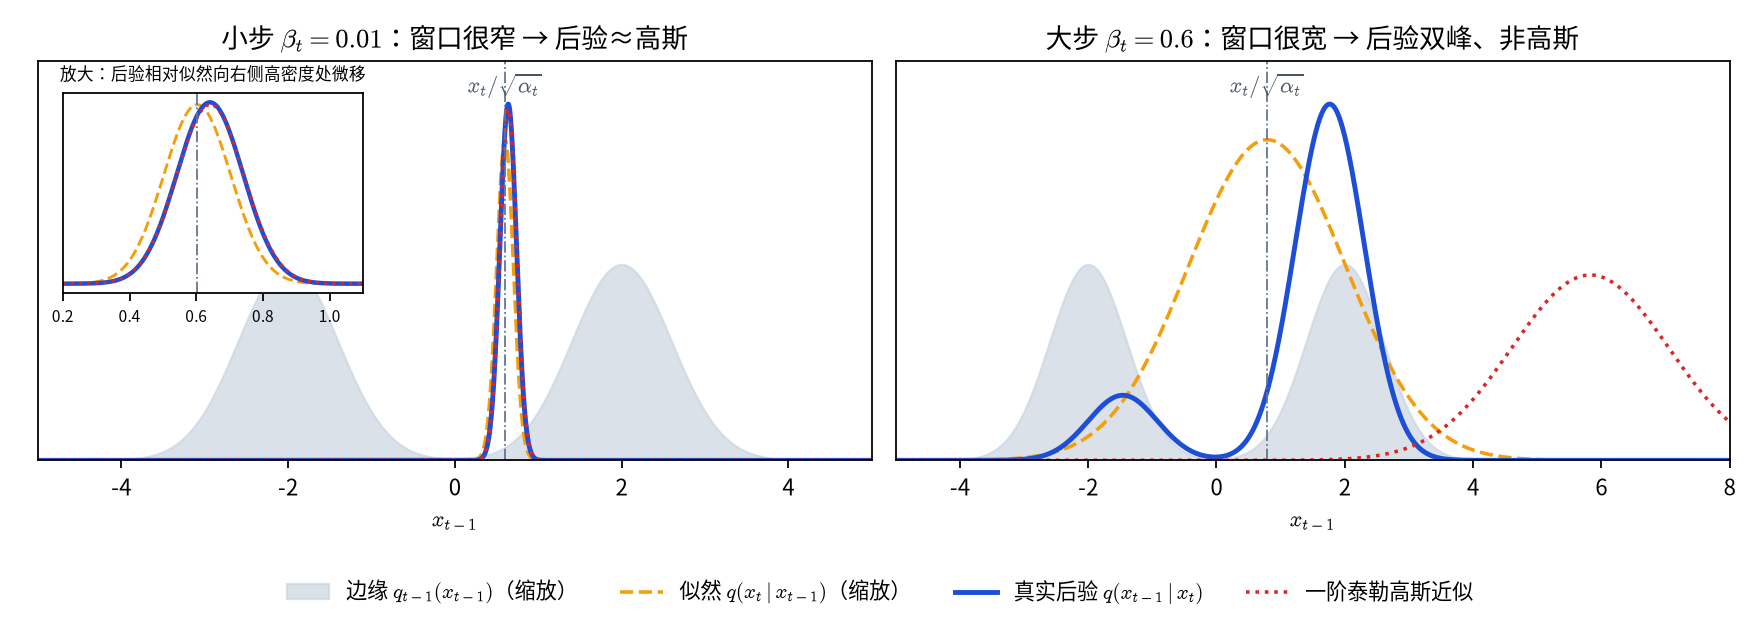
\includegraphics[width=0.98\textwidth]{figures/fig5_reverse_gaussian_smallstep.png}
  \caption{一维示意：$q_{t-1}$ 为双峰混合（灰），真实后验 $q(x_{t-1}\mid x_t)\propto$ 似然 $\times\,q_{t-1}$（蓝），一阶泰勒高斯近似 \eqref{eq:rev-gauss-raw}（红点线）。
  左：$\beta_t=0.01$，窗口远窄于 $q_{t-1}$ 的变化尺度，近似几乎精确；右：$\beta_t=0.6$，窗口覆盖两个峰，真实后验双峰，高斯近似完全失效。}
  \label{fig:smallstep}
\end{figure}

\paragraph{第 4 步：大步为什么失效。}若 $\beta_t$ 很大，窗口宽度 $\sqrt{\beta_t}$ 与 $\ell_{t-1}$ 可比甚至更大：窗口里 $\log q_{t-1}$ 的弯曲、多峰结构都会显现，
三阶以上的项不再可忽略，真实后验可以是偏斜的甚至多峰的（图~\ref{fig:smallstep} 右）。此时用单个高斯建模反向一步会产生系统误差，
表现为样本模糊或模式混合。这就是：
\begin{itemize}[leftmargin=1.6em,itemsep=1pt]
  \item DDPM 采用 $T\approx1000$ 个小步（每步 $\beta_t\le0.02$），让每一步的高斯近似都足够准确；
  \item 想用很少步数采样时需要别的办法：DDIM、概率流 ODE 等确定性求解器（不再需要逐步的高斯后验假设）、知识蒸馏 / 一致性模型，
        或像 Denoising Diffusion GAN（Xiao et al., ICLR 2022）那样用可表达多峰的生成器来建模大步的反向转移。
\end{itemize}
\textbf{形式化结论。}Feller（1949）关于扩散过程的经典结果、以及 Sohl-Dickstein et al.（2015）在扩散生成模型中的论证表明：
当步长趋于零时，高斯扩散的反向过程与前向过程具有\emph{相同的函数形式}（反向也是高斯转移）；上面的泰勒论证正是这一连续极限结论的离散、直观版本。

\paragraph{第 5 步：均值里出现了得分——与 \texorpdfstring{$\eps$}{eps} 形式和 SDE 的联系。}
式 \eqref{eq:rev-gauss} 的均值含得分 $\nabla\log q_t(\x_t)$。它与噪声的关系可逐行推出：边缘是对 $\x_0$ 的积分 $q_t(\x_t)=\int q(\x_t\mid\x_0)\,q(\x_0)\,\mathrm{d}\x_0$，
对 $\x_t$ 求梯度（梯度可移入积分），并用 $\nabla q=q\,\nabla\log q$：
\begin{align}
  \nabla q_t(\x_t)&=\int \nabla_{\x_t}q(\x_t\mid\x_0)\,q(\x_0)\,\mathrm{d}\x_0
   =\int q(\x_t\mid\x_0)\,q(\x_0)\;\nabla_{\x_t}\log q(\x_t\mid\x_0)\,\mathrm{d}\x_0 , \notag\\
  \nabla\log q_t(\x_t)=\frac{\nabla q_t(\x_t)}{q_t(\x_t)}
   &=\int \underbrace{\frac{q(\x_t\mid\x_0)\,q(\x_0)}{q_t(\x_t)}}_{=\,q(\x_0\mid\x_t)\ \text{（贝叶斯）}}\nabla_{\x_t}\log q(\x_t\mid\x_0)\,\mathrm{d}\x_0 . \notag
\end{align}
而由 \eqref{eq:iso-gauss}，$\log q(\x_t\mid\x_0)=-\frac{\|\x_t-\sqrt{\abar_t}\x_0\|^2}{2(1-\abar_t)}+\mathrm{const}$，梯度为 $-\frac{\x_t-\sqrt{\abar_t}\x_0}{1-\abar_t}=-\frac{\eps}{\sqrt{1-\abar_t}}$（用 \eqref{eq:closed}）。合起来：
\begin{equation}
  \nabla\log q_t(\x_t)=\E_{q(\x_0\mid\x_t)}\!\big[\nabla_{\x_t}\log q(\x_t\mid\x_0)\big]
  =-\frac{\E[\eps\mid\x_t]}{\sqrt{1-\abar_t}},
  \label{eq:marginal-score}
\end{equation}
其中用到了第六节式 \eqref{eq:eps-score} 的条件得分 $-\eps/\sqrt{1-\abar_t}$。代入 \eqref{eq:rev-gauss}：
\begin{equation}
  \text{均值}\approx\frac{1}{\sqrt{\alpha_t}}\Big(\x_t-\frac{\beta_t}{\sqrt{1-\abar_t}}\,\E[\eps\mid\x_t]\Big),
\end{equation}
与 3.5 节的噪声参数化 \eqref{eq:mu-eps} 形式\emph{完全一致}，只需 $\epst(\x_t,t)\approx\E[\eps\mid\x_t]$——而这恰是简化损失 $\Lsimple$（均方误差）的最优解。
从「小步高斯近似」与从「贝叶斯精确后验 + 对 $\x_0$ 取平均」两条路得到同一个答案。

同样，第六节 VP-SDE \eqref{eq:vp-sde} 的反向 SDE \eqref{eq:rev-sde} 以步长 $1$（离散时间单位，$\beta(t)\,\mathrm{d}t\to\beta_t$）做一步 Euler–Maruyama：
\begin{equation}
  \x_{t-1}=\x_t+\Big(\tfrac12\beta_t\,\x_t+\beta_t\,\nabla\log q_t(\x_t)\Big)+\sqrt{\beta_t}\,\mathbf{z}
  \approx\frac{1}{\sqrt{\alpha_t}}\big(\x_t+\beta_t\nabla\log q_t(\x_t)\big)+\sqrt{\beta_t}\,\mathbf{z},
\end{equation}
（用到 $1+\frac12\beta_t=\alpha_t^{-1/2}+O(\beta_t^2)$），恰好就是从 \eqref{eq:rev-gauss} 中采样。离散的「小步高斯」与连续的「反向 SDE」是同一件事。

\subsection{可学习的反向模型}
于是用参数化高斯族去拟合反向链：
\begin{keybox}
\begin{align}
  p_\theta(\x_{0:T}) &= p(\x_T)\prod_{t=1}^{T} p_\theta(\x_{t-1}\mid\x_t), \label{eq:rev-joint}\\
  p(\x_T) &= \N(\x_T;\ \mathbf{0},\ \I), \\
  p_\theta(\x_{t-1}\mid\x_t) &= \N\!\left(\x_{t-1};\ \mutheta(\x_t,t),\ \sigma_t^2\I\right). \label{eq:rev-step}
\end{align}
\end{keybox}
一般形式中协方差可写为 $\boldsymbol{\Sigma}_\theta(\x_t,t)$；DDPM 将其固定为与时间相关的各向同性常数 $\sigma_t^2\I$（取 $\sigma_t^2=\beta_t$ 或 $\sigma_t^2=\btil_t$），只学习均值 $\mutheta$。

\begin{whybox}
\textbf{为什么方差可以固定为 $\beta_t$ 或 $\btil_t$？}Ho et al.（2020）指出这两个取值分别是反向方差的两个极端：
若 $\x_0\sim\N(\mathbf{0},\I)$，最优方差是 $\beta_t$；若 $\x_0$ 是一个确定的点，最优方差是 $\btil_t$（下文式 \eqref{eq:post-var}）。
真实数据介于两者之间，而 $\btil_t\le\beta_t$ 且当 $T$ 很大时两者在绝大多数 $t$ 上几乎相等，实验上样本质量相近。
固定方差还有两个好处：(i) KL 散度退化为纯粹的均值平方误差（见 4.2 节），训练目标更简单、更稳定；
(ii) Ho et al. 报告直接学习对角方差会导致训练不稳定、样本更差（后续 Nichol \& Dhariwal 2021 通过在 $\beta_t$ 与 $\btil_t$ 之间插值学习方差改进了对数似然）。
\end{whybox}

\subsection{从贝叶斯出发：推导 \texorpdfstring{$q(\x_{t-1}\mid\x_t,\x_0)$}{q(x\_{t-1}|x\_t,x\_0)}}
下面一步一步推导这个「标准答案」后验。所有向量运算都是逐坐标独立的（协方差均为 $\cdot\,\I$），
记 $\|\mathbf{v}\|^2=\mathbf{v}^\top\mathbf{v}$。

\paragraph{第 1 步：贝叶斯公式。}在条件 $\x_0$ 下，对 $\x_{t-1}$ 与 $\x_t$ 应用贝叶斯公式：
\begin{equation}
  q(\x_{t-1}\mid\x_t,\x_0)=\frac{q(\x_t\mid\x_{t-1},\x_0)\;q(\x_{t-1}\mid\x_0)}{q(\x_t\mid\x_0)} .
  \label{eq:bayes}
\end{equation}

\paragraph{第 2 步：马尔可夫性。}前向链是马尔可夫的：给定 $\x_{t-1}$ 后，$\x_t$ 与更早的 $\x_0$ 条件独立，因此
\begin{equation}
  q(\x_t\mid\x_{t-1},\x_0)=q(\x_t\mid\x_{t-1})=\N\!\left(\x_t;\ \sqrt{\alpha_t}\,\x_{t-1},\ \beta_t\I\right).
  \label{eq:markov}
\end{equation}
\begin{whybox}
\textbf{为什么要用马尔可夫性？}贝叶斯公式里的似然项原本是 $q(\x_t\mid\x_{t-1},\x_0)$，我们并没有直接定义它；
马尔可夫性把它化成了我们定义过的单步转移 \eqref{eq:fwd-step}。式 \eqref{eq:bayes} 的另外两项则正是闭式边缘 \eqref{eq:closed-dist}（分别取 $t-1$ 与 $t$）。
于是右边三项\emph{全部已知且都是高斯}。
\end{whybox}

\paragraph{第 3 步：写出三个高斯密度。}利用 $\N(\x;\mathbf{m},s\I)\propto\exp\!\big(-\frac{1}{2}\frac{\|\x-\mathbf{m}\|^2}{s}\big)$（即式 \eqref{eq:iso-gauss}，3.2 节 (1b) 已推导）：
\begin{align}
  q(\x_t\mid\x_{t-1}) &\propto \exp\!\Big(-\frac12\,\frac{\|\x_t-\sqrt{\alpha_t}\,\x_{t-1}\|^2}{\beta_t}\Big), \\
  q(\x_{t-1}\mid\x_0) &\propto \exp\!\Big(-\frac12\,\frac{\|\x_{t-1}-\sqrt{\abar_{t-1}}\,\x_0\|^2}{1-\abar_{t-1}}\Big), \\
  q(\x_t\mid\x_0) &\propto \exp\!\Big(-\frac12\,\frac{\|\x_t-\sqrt{\abar_t}\,\x_0\|^2}{1-\abar_t}\Big).
\end{align}
（三式都由各向同性高斯密度 \eqref{eq:iso-gauss} 得到；省略的系数 $(2\pi\beta_t)^{-d/2}$、$(2\pi(1-\abar_{t-1}))^{-d/2}$、$(2\pi(1-\abar_t))^{-d/2}$ 都不含 $\x_{t-1}$。）
代入 \eqref{eq:bayes}：分子两个指数相乘 $=$ 指数相加；除以分母 $\exp(-\frac12 Q)$ 等于乘以 $\exp(+\frac12 Q)$，所以分母的平方项在方括号里带\emph{负号}。把所有与 $\x_{t-1}$ 无关的归一化常数吸收进比例号：
\begin{equation}
  q(\x_{t-1}\mid\x_t,\x_0)\propto
  \exp\!\Big(-\frac12\Big[
    \frac{\|\x_t-\sqrt{\alpha_t}\,\x_{t-1}\|^2}{\beta_t}
   +\frac{\|\x_{t-1}-\sqrt{\abar_{t-1}}\,\x_0\|^2}{1-\abar_{t-1}}
   -\frac{\|\x_t-\sqrt{\abar_t}\,\x_0\|^2}{1-\abar_t}
  \Big]\Big).
  \label{eq:post-exp}
\end{equation}
注意：这里的变量是 $\x_{t-1}$；$\x_t$ 与 $\x_0$ 都是给定的常量。

\paragraph{第 4 步：展开指数。}逐项展开平方（$\|\mathbf{a}-\mathbf{b}\|^2=\|\mathbf{a}\|^2-2\mathbf{a}^\top\mathbf{b}+\|\mathbf{b}\|^2$）：
\begin{align}
  \frac{\|\x_t-\sqrt{\alpha_t}\,\x_{t-1}\|^2}{\beta_t}
   &= \frac{\|\x_t\|^2}{\beta_t}-\frac{2\sqrt{\alpha_t}}{\beta_t}\,\x_t^\top\x_{t-1}+\frac{\alpha_t}{\beta_t}\,\|\x_{t-1}\|^2, \\
  \frac{\|\x_{t-1}-\sqrt{\abar_{t-1}}\,\x_0\|^2}{1-\abar_{t-1}}
   &= \frac{\|\x_{t-1}\|^2}{1-\abar_{t-1}}-\frac{2\sqrt{\abar_{t-1}}}{1-\abar_{t-1}}\,\x_0^\top\x_{t-1}+\frac{\abar_{t-1}\|\x_0\|^2}{1-\abar_{t-1}}, \\
  \frac{\|\x_t-\sqrt{\abar_t}\,\x_0\|^2}{1-\abar_t} &= C_1(\x_t,\x_0)\qquad\text{（与 $\x_{t-1}$ 无关）}.
\end{align}

\paragraph{第 5 步：按 $\x_{t-1}$ 的二次项、一次项、常数项归类。}方括号内整体等于
\begin{equation}
  \underbrace{\Big(\frac{\alpha_t}{\beta_t}+\frac{1}{1-\abar_{t-1}}\Big)}_{\eqqcolon\,A_t}\|\x_{t-1}\|^2
  \;-\;2\,\underbrace{\Big(\frac{\sqrt{\alpha_t}}{\beta_t}\,\x_t+\frac{\sqrt{\abar_{t-1}}}{1-\abar_{t-1}}\,\x_0\Big)}_{\eqqcolon\,\mathbf{b}_t}{}^{\!\top}\x_{t-1}
  \;+\;C_2(\x_t,\x_0),
  \label{eq:quad-form}
\end{equation}
其中 $C_2=\frac{\|\x_t\|^2}{\beta_t}+\frac{\abar_{t-1}\|\x_0\|^2}{1-\abar_{t-1}}-C_1$ 不含 $\x_{t-1}$。

\paragraph{第 6 步：配方。}对任意 $A>0$，
\begin{equation}
  A\|\x\|^2-2\mathbf{b}^\top\x
  = A\,\Big\|\x-\frac{\mathbf{b}}{A}\Big\|^2-\frac{\|\mathbf{b}\|^2}{A}
  = \frac{\|\x-\mathbf{b}/A\|^2}{1/A}+\text{常数}.
\end{equation}
因此 $q(\x_{t-1}\mid\x_t,\x_0)\propto\exp\!\big(-\frac12\,\|\x_{t-1}-\mathbf{b}_t/A_t\|^2\big/(1/A_t)\big)$，
它是高斯，\textbf{方差} $=1/A_t$，\textbf{均值} $=\mathbf{b}_t/A_t$：
\begin{equation}
  \btil_t=\frac{1}{A_t},\qquad \mut_t(\x_t,\x_0)=\frac{\mathbf{b}_t}{A_t}=\btil_t\,\mathbf{b}_t .
  \label{eq:read-off}
\end{equation}
\begin{whybox}
\textbf{为什么只看 $\x_{t-1}$ 的二次项和一次项？}高斯的对数密度是变量的二次函数：
$-\frac{1}{2s}\|\x-\mathbf{m}\|^2=-\frac12\big(\frac1s\|\x\|^2-\frac{2}{s}\mathbf{m}^\top\x\big)+\text{常数}$。
二次项系数给出精度 $1/s$，一次项系数给出 $\mathbf{m}/s$；常数项只影响归一化，最后会被自动补齐。
这样就不必去算繁琐的归一化常数。
\end{whybox}

\paragraph{第 7 步：化简方差 $\btil_t$。}通分并利用 $\beta_t=1-\alpha_t$、$\alpha_t\abar_{t-1}=\abar_t$：
\begin{align}
  \frac{1}{\btil_t}=A_t
  &= \frac{\alpha_t}{\beta_t}+\frac{1}{1-\abar_{t-1}}
   = \frac{\alpha_t(1-\abar_{t-1})+\beta_t}{\beta_t(1-\abar_{t-1})} \notag\\
  &= \frac{\alpha_t-\alpha_t\abar_{t-1}+1-\alpha_t}{\beta_t(1-\abar_{t-1})}
   = \frac{1-\abar_t}{\beta_t(1-\abar_{t-1})},
  \label{eq:precision}
\end{align}
所以
\begin{keybox}
\begin{equation}
  \btil_t=\frac{1-\abar_{t-1}}{1-\abar_t}\,\beta_t .
  \label{eq:post-var}
\end{equation}
\end{keybox}

\paragraph{第 8 步：化简均值 $\mut_t$。}由 \eqref{eq:read-off}，把 $\btil_t$ 乘进 $\mathbf{b}_t$ 的两项：
\begin{align}
  \mut_t(\x_t,\x_0)
  &= \frac{(1-\abar_{t-1})\beta_t}{1-\abar_t}\Big(\frac{\sqrt{\alpha_t}}{\beta_t}\,\x_t+\frac{\sqrt{\abar_{t-1}}}{1-\abar_{t-1}}\,\x_0\Big) \notag\\
  &= \frac{\sqrt{\alpha_t}\,(1-\abar_{t-1})}{1-\abar_t}\,\x_t+\frac{\sqrt{\abar_{t-1}}\,\beta_t}{1-\abar_t}\,\x_0 .
\end{align}
整理成结论：
\begin{keybox}
\begin{align}
  q(\x_{t-1}\mid\x_t,\x_0) &= \N\!\left(\x_{t-1};\ \mut_t(\x_t,\x_0),\ \btil_t\I\right), \label{eq:post}\\
  \mut_t(\x_t,\x_0) &= \frac{\sqrt{\abar_{t-1}}\,\beta_t}{1-\abar_t}\,\x_0
                     + \frac{\sqrt{\alpha_t}\,(1-\abar_{t-1})}{1-\abar_t}\,\x_t. \label{eq:post-mean}
\end{align}
\end{keybox}
\begin{whybox}
\textbf{如何理解这个结果？}(1) $\mut_t$ 是 $\x_0$（「干净图像在哪」）与 $\x_t$（「当前所在位置」）的加权组合：
$\x_0$ 的权重随 $\beta_t$ 增大，$\x_t$ 的权重随 $1-\abar_{t-1}$ 增大。
(2) 两个高斯「证据」（来自 $\x_t$ 的似然、来自 $\x_0$ 的先验）相乘，精度相加：$1/\btil_t=\alpha_t/\beta_t+1/(1-\abar_{t-1})$，
所以 $\btil_t$ 比任何单方证据的方差都小，且 $\btil_t\le\beta_t$。
(3) \textbf{自检：}$t=1$ 时 $\abar_0=1$，得 $\btil_1=0$、$\mut_1=\x_0$——已知 $\x_0$ 时，「上一步」就是 $\x_0$ 本身，完全合理。
\end{whybox}

\subsection{把 \texorpdfstring{$\mut_t$}{mu-tilde\_t} 改写成噪声 \texorpdfstring{$\eps$}{eps} 的形式}
采样时 $\x_0$ 是未知的，所以 \eqref{eq:post-mean} 不能直接用。但由闭式 \eqref{eq:closed}（即重参数化，见 \ref{sec:reparam} 节用法 (3c)-(iii)），给定 $\x_t$ 时 $\x_0$ 与 $\eps$ 一一对应：
\begin{equation}
  \x_t=\sqrt{\abar_t}\,\x_0+\sqrt{1-\abar_t}\,\eps
  \quad\Longleftrightarrow\quad
  \x_0=\frac{1}{\sqrt{\abar_t}}\Big(\x_t-\sqrt{1-\abar_t}\,\eps\Big).
  \label{eq:x0-from-eps}
\end{equation}
把 \eqref{eq:x0-from-eps} 代入 \eqref{eq:post-mean}，并注意 $\sqrt{\abar_{t-1}}/\sqrt{\abar_t}=1/\sqrt{\alpha_t}$：
\begin{align}
  \mut_t
  &= \frac{\sqrt{\abar_{t-1}}\,\beta_t}{1-\abar_t}\cdot\frac{1}{\sqrt{\abar_t}}\Big(\x_t-\sqrt{1-\abar_t}\,\eps\Big)
     + \frac{\sqrt{\alpha_t}\,(1-\abar_{t-1})}{1-\abar_t}\,\x_t \notag\\
  &= \frac{\beta_t}{\sqrt{\alpha_t}\,(1-\abar_t)}\,\x_t
     - \frac{\beta_t\sqrt{1-\abar_t}}{\sqrt{\alpha_t}\,(1-\abar_t)}\,\eps
     + \frac{\sqrt{\alpha_t}\,(1-\abar_{t-1})}{1-\abar_t}\,\x_t \notag\\
  &= \frac{\beta_t+\alpha_t(1-\abar_{t-1})}{\sqrt{\alpha_t}\,(1-\abar_t)}\,\x_t
     - \frac{\beta_t}{\sqrt{\alpha_t}\,\sqrt{1-\abar_t}}\,\eps
     \qquad\Big(\text{第三项上下同乘 }\sqrt{\alpha_t}\Big) \notag\\
  &= \frac{1-\abar_t}{\sqrt{\alpha_t}\,(1-\abar_t)}\,\x_t
     - \frac{\beta_t}{\sqrt{\alpha_t}\,\sqrt{1-\abar_t}}\,\eps
     \qquad\Big(\text{分子同 \eqref{eq:precision}：}\beta_t+\alpha_t-\abar_t=1-\abar_t\Big) \notag
\end{align}
\begin{keybox}
\begin{equation}
  \mut_t(\x_t,\x_0)=\frac{1}{\sqrt{\alpha_t}}\left(\x_t-\frac{\beta_t}{\sqrt{1-\abar_t}}\,\eps\right),
  \qquad \eps=\frac{\x_t-\sqrt{\abar_t}\,\x_0}{\sqrt{1-\abar_t}} .
  \label{eq:mut-eps}
\end{equation}
\end{keybox}
现在「理想均值」里唯一未知的是 $\x_t$ 中所含的噪声 $\eps$。用网络 $\epst(\x_t,t)$ 预测它，就得到可学习的均值：
\begin{keybox}
\begin{equation}
  \mutheta(\x_t,t) = \frac{1}{\sqrt{\alpha_t}}\left(\x_t-\frac{\beta_t}{\sqrt{1-\abar_t}}\,\epst(\x_t,t)\right).
  \label{eq:mu-eps}
\end{equation}
\end{keybox}
网络的任务变成：看见带噪样本 $\x_t$ 与时间 $t$，输出「当初加进去的那份噪声」$\eps$ 的估计。

\subsection{为什么预测噪声 \texorpdfstring{$\eps$}{eps}，而不是 \texorpdfstring{$\x_0$}{x\_0} 或 \texorpdfstring{$\mut_t$}{mu}}
\begin{whybox}
\begin{enumerate}[leftmargin=1.5em,itemsep=2pt]
  \item \textbf{三者在数学上等价。}给定 $(\x_t,t)$，由 \eqref{eq:x0-from-eps} 与 \eqref{eq:mut-eps}，$\eps$、$\x_0$、$\mut_t$ 之间是可逆的仿射变换：
        $\hat{\x}_0=(\x_t-\sqrt{1-\abar_t}\,\epst)/\sqrt{\abar_t}$。所以选哪个只是\emph{重参数化}，不改变模型表达能力；差别在于优化难度。
  \item \textbf{尺度统一、数值稳定。}目标 $\eps\sim\N(\mathbf{0},\I)$ 对所有 $t$ 都是单位方差，网络输出的尺度不随 $t$ 变化。
        若预测 $\mut_t$：小 $t$ 时 $\mut_t\approx\x_t$，网络要输出「几乎恒等 + 极小修正」，修正量淹没在大信号里；
        若预测 $\x_0$：大 $t$ 时几乎看不到信号，再通过 $1/\sqrt{\abar_t}$ 等系数传播时误差会被放大。
  \item \textbf{类似残差学习。}式 \eqref{eq:mu-eps} 中 $\mutheta=\frac{1}{\sqrt{\alpha_t}}\x_t-(\text{小修正})$，网络只负责「修正量」部分，这与 ResNet 学残差的思路一致。
  \item \textbf{与得分直接对应。}$\nabla_{\x_t}\log q(\x_t\mid\x_0)=-\eps/\sqrt{1-\abar_t}$（第六节式 \eqref{eq:eps-score}），
        预测噪声就是在估计（缩放后的）得分，训练目标即多噪声尺度下的去噪得分匹配。
  \item \textbf{实验结论。}Ho et al.（2020，表 2）比较过预测 $\mut$ 与预测 $\eps$：$\eps$ 预测配合简化损失得到了最好的 FID。
\end{enumerate}
\end{whybox}

% ======================== 四 ========================
\section{训练目标：从变分下界到简化 MSE}

\subsection{极大似然与 ELBO}
我们希望最大化 $\E_{q(\x_0)}[\log p_\theta(\x_0)]$。引入潜变量 $\x_{1:T}$ 后，
由 Jensen 不等式得到变分下界（ELBO）；习惯上最小化其相反数 $\LVLB$（负对数似然的上界）：
\begin{keybox}
\begin{equation}
  -\log p_\theta(\x_0) \;\le\; \E_{q(\x_{1:T}\mid\x_0)}\!\left[-\log\frac{p_\theta(\x_{0:T})}{q(\x_{1:T}\mid\x_0)}\right] \;\eqqcolon\; \LVLB .
  \label{eq:vlb}
\end{equation}
\end{keybox}
\begin{whybox}
\textbf{为什么不直接最大化 $\log p_\theta(\x_0)$？}$p_\theta(\x_0)=\int p_\theta(\x_{0:T})\,\mathrm{d}\x_{1:T}$ 是对 $T$ 个高维变量的积分，无法计算。
借助前向过程 $q(\x_{1:T}\mid\x_0)$ 作为「变分分布」（且它固定、易采样），就能把对数似然换成可蒙特卡洛估计的上界 $\LVLB$；压低上界即间接提高似然。
\end{whybox}

\textbf{分解推导。}由 \eqref{eq:fwd-joint} 与 \eqref{eq:rev-joint}，
\begin{equation}
  \LVLB=\E_q\Big[-\log p(\x_T)-\sum_{t=2}^{T}\log\frac{p_\theta(\x_{t-1}\mid\x_t)}{q(\x_t\mid\x_{t-1})}-\log\frac{p_\theta(\x_0\mid\x_1)}{q(\x_1\mid\x_0)}\Big].
\end{equation}
关键一步：对 $t\ge 2$ 用马尔可夫性和贝叶斯公式 \eqref{eq:bayes}，把前向转移「翻转」成后验：
\begin{equation}
  q(\x_t\mid\x_{t-1})=q(\x_t\mid\x_{t-1},\x_0)=\frac{q(\x_{t-1}\mid\x_t,\x_0)\,q(\x_t\mid\x_0)}{q(\x_{t-1}\mid\x_0)} .
\end{equation}
代入后，$\sum_{t=2}^T\log\frac{q(\x_t\mid\x_0)}{q(\x_{t-1}\mid\x_0)}=\log\frac{q(\x_T\mid\x_0)}{q(\x_1\mid\x_0)}$ 逐项相消（望远镜求和），
其中 $q(\x_1\mid\x_0)$ 与最后一项中的 $q(\x_1\mid\x_0)$ 抵消，剩下
\begin{equation}
  \LVLB=\E_q\Big[\log\frac{q(\x_T\mid\x_0)}{p(\x_T)}+\sum_{t=2}^{T}\log\frac{q(\x_{t-1}\mid\x_t,\x_0)}{p_\theta(\x_{t-1}\mid\x_t)}-\log p_\theta(\x_0\mid\x_1)\Big],
\end{equation}
每个对数比在期望下就是一个 KL 散度，得到常见分解（符号随文献略有出入）：
\begin{align}
  \LVLB &= L_T + \sum_{t=2}^{T} L_{t-1} + L_0, \label{eq:vlb-decomp}\\
  L_T &= \E_q\!\left[\KL{q(\x_T\mid\x_0)}{p(\x_T)}\right] && \text{（前向末端 vs 标准正态先验，与 $\theta$ 无关且很小）} \notag\\
  L_{t-1} &= \E_q\!\left[\KL{q(\x_{t-1}\mid\x_t,\x_0)}{p_\theta(\x_{t-1}\mid\x_t)}\right] && \notag\\
  L_0 &= -\E_q\!\left[\log p_\theta(\x_0\mid\x_1)\right] && \text{（离散像素时常用离散解码器似然）} \notag
\end{align}

\begin{whybox}
\textbf{为什么要让 $p_\theta(\x_{t-1}\mid\x_t)$ 去匹配后验 $q(\x_{t-1}\mid\x_t,\x_0)$？}这不是人为的选择，而是 ELBO 分解\emph{自动}给出的：
最小化 $\LVLB$ 就是最小化每个 $L_{t-1}$ 中的 KL。之所以出现「条件在 $\x_0$ 上」的后验，是因为上面翻转前向转移时引入了 $\x_0$，
而这正好让比较对象变成可解析计算的高斯（3.4 节）。

\textbf{但 $p_\theta$ 看不到 $\x_0$，怎么匹配？}对固定的 $\x_t$，不同的 $\x_0$ 给出不同的 $\mut_t$；网络只能输出一个 $\mutheta(\x_t,t)$。
平方误差回归的最优解是条件期望：$\mutheta^\star(\x_t,t)=\E_{q(\x_0\mid\x_t)}\!\big[\mut_t(\x_t,\x_0)\big]$，
这恰好是真实反向转移 $q(\x_{t-1}\mid\x_t)$ 的均值。所以「对带噪标签做回归」最终学到的就是那个我们算不出来的真实反向均值。
\end{whybox}

\subsection{高斯 KL 化为均值匹配}
因为 $q(\x_{t-1}\mid\x_t,\x_0)$ 与 $p_\theta(\x_{t-1}\mid\x_t)$ 都是各向同性高斯，且协方差固定为 $\btil_t\I$ 与 $\sigma_t^2\I$，
利用两个高斯的 KL 公式 $D_{\mathrm{KL}}\big(\N(\mathbf{m}_1,s_1\I)\,\|\,\N(\mathbf{m}_2,s_2\I)\big)=\frac{\|\mathbf{m}_1-\mathbf{m}_2\|^2}{2s_2}+\frac d2\big(\frac{s_1}{s_2}-1-\log\frac{s_1}{s_2}\big)$（$d$ 为维数），
后一项与 $\theta$ 无关，故 KL 散度除去常数 $C$ 外，就是两均值之差的加权平方：
\begin{equation}
  L_{t-1} = \E_q\!\left[\frac{1}{2\sigma_t^2}\left\|\mut_t(\x_t,\x_0)-\mutheta(\x_t,t)\right\|^2\right] + C .
  \label{eq:mean-match}
\end{equation}

\subsection{换成 \texorpdfstring{$\eps$}{eps} 参数化后的简化目标}
把 $\mutheta$ 用 \eqref{eq:mu-eps} 参数化，并做重参数化 $\x_t=\sqrt{\abar_t}\,\x_0+\sqrt{1-\abar_t}\,\eps$（\ref{sec:reparam} 节），
由 \eqref{eq:mut-eps} 与 \eqref{eq:mu-eps}，两均值中 $\x_t$ 项相同、直接相消：
\begin{equation}
  \mut_t-\mutheta=\frac{1}{\sqrt{\alpha_t}}\cdot\frac{\beta_t}{\sqrt{1-\abar_t}}\big(\epst(\x_t,t)-\eps\big),
  \qquad
  \frac{\|\mut_t-\mutheta\|^2}{2\sigma_t^2}=\frac{\beta_t^2}{2\sigma_t^2\,\alpha_t\,(1-\abar_t)}\,\|\eps-\epst\|^2 .
\end{equation}
于是均值匹配等价于加权的噪声匹配：
\begin{equation}
  L_{t-1} - C = \E_{\x_0,\eps}\!\left[\frac{\beta_t^2}{2\sigma_t^2\,\alpha_t\,(1-\abar_t)}
     \left\|\eps-\epst\!\left(\sqrt{\abar_t}\,\x_0+\sqrt{1-\abar_t}\,\eps,\ t\right)\right\|^2\right].
  \label{eq:weighted}
\end{equation}
DDPM 进一步丢掉随 $t$ 变化的权重，得到实践中极其好用的简化损失：
\begin{keybox}
\begin{equation}
  \Lsimple(\theta) = \E_{t,\x_0,\eps}\!\left[\left\|\eps-\epst\!\left(\sqrt{\abar_t}\,\x_0+\sqrt{1-\abar_t}\,\eps,\ t\right)\right\|^2\right],
  \label{eq:lsimple}
\end{equation}
\[
  t\sim\mathrm{Uniform}\{1,\dots,T\},\qquad \eps\sim\N(\mathbf{0},\I),\qquad \x_0\sim q(\x_0)\ \text{（数据）}.
\]
\end{keybox}

\begin{whybox}
\textbf{为什么可以丢掉权重 $\lambda_t=\frac{\beta_t^2}{2\sigma_t^2\alpha_t(1-\abar_t)}$？}
(1) 取 $\sigma_t^2=\beta_t$ 时 $\lambda_t=\frac{\beta_t}{2\alpha_t(1-\abar_t)}$：$t=1$ 时 $1-\abar_1=\beta_1$，$\lambda_1\approx\frac12$；
$t$ 较大时 $1-\abar_t\approx 1$，$\lambda_t\approx\beta_t/2\sim 10^{-2}$。也就是说 ELBO 权重\emph{偏重小 $t$}（几乎没有噪声、本来就容易的去噪）。
(2) 去掉权重相当于\emph{相对提高大 $t$ 的权重}，让网络把容量用在更难的去噪任务上；Ho et al. 实验中这显著提升了样本质量（FID），代价是对数似然略差。
(3) 去权重后各项的数值尺度一致（都是单位方差噪声的 MSE），梯度更平稳，实现也最简单。
(4) 它仍是「各噪声水平上的去噪得分匹配之和」，只是换了一种加权，因此依然是合理的训练目标。
\end{whybox}

\begin{notebox}
\textbf{推导链小结：}似然 $\to$ ELBO $\to$ 逐步 KL $\to$ 高斯均值匹配 $\to$ $\eps$ 参数化 $\to$
（可选）去权重得到 $\Lsimple$。简化损失不等于精确的 $\LVLB$，
但在图像生成上往往更稳、样本质量更好，因而成为事实标准。
\end{notebox}

\setcounter{figure}{2}% 与图片内嵌标题编号保持一致
\begin{figure}[H]
  \centering
  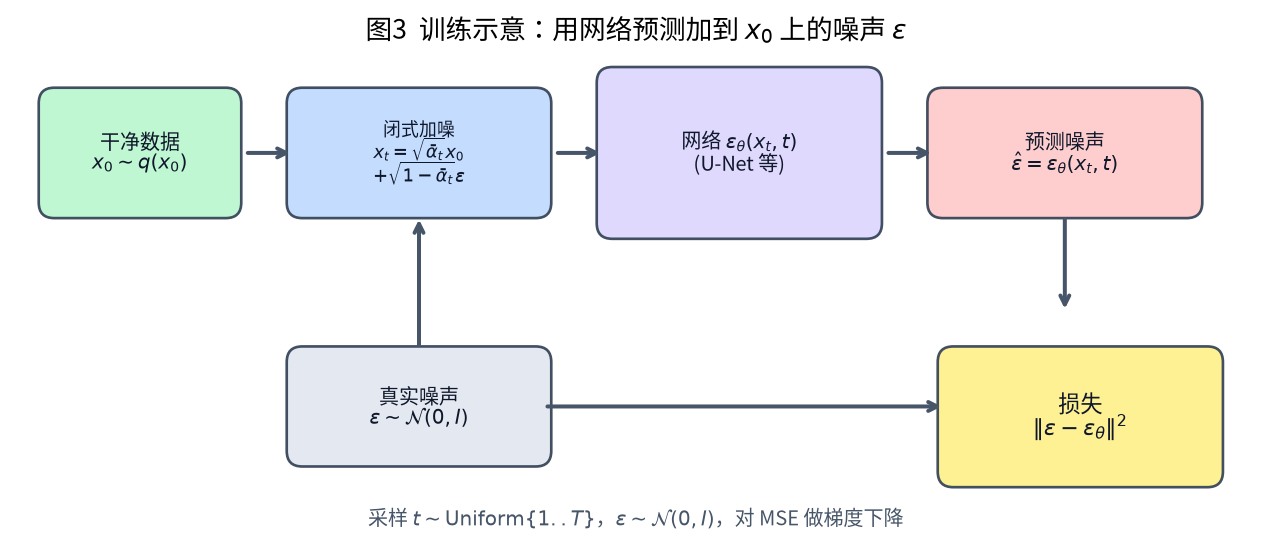
\includegraphics[width=0.86\textwidth]{figures/fig3_training_schematic.png}
  \caption{训练流程图：闭式构造 $\x_t$，网络预测 $\eps$，对 MSE 反向传播}
  \label{fig:train}
\end{figure}

\subsection{训练算法（伪代码）}
\begin{algorithm}[H]
  \caption{DDPM 训练（Ho et al., 2020, Algorithm 1）}
  \label{alg:train}
  \begin{algorithmic}[1]
    \Repeat
      \State $\x_0\sim q(\x_0)$ \Comment{从训练集采样}
      \State $t\sim\mathrm{Uniform}\{1,\dots,T\}$
      \State $\eps\sim\N(\mathbf{0},\I)$
      \State $\x_t\gets\sqrt{\abar_t}\,\x_0+\sqrt{1-\abar_t}\,\eps$ \Comment{重参数化闭式加噪，式 \eqref{eq:closed}}
      \State 对 $\nabla_\theta\left\|\eps-\epst(\x_t,t)\right\|^2$ 做一步梯度下降
    \Until{收敛}
  \end{algorithmic}
\end{algorithm}

% ======================== 五 ========================
\section{采样算法（DDPM）}
训练完成后，生成新样本不需要 $\x_0$，只需从先验噪声出发迭代应用学习到的反向转移 \eqref{eq:rev-step}。

\begin{algorithm}[H]
  \caption{DDPM 祖先采样（ancestral sampling）}
  \label{alg:sample}
  \begin{algorithmic}[1]
    \State $\x_T\sim\N(\mathbf{0},\I)$
    \For{$t=T,T-1,\dots,1$}
      \State $\hat{\eps}\gets\epst(\x_t,t)$
      \State $\boldsymbol{\mu}\gets\dfrac{1}{\sqrt{\alpha_t}}\Bigl(\x_t-\dfrac{\beta_t}{\sqrt{1-\abar_t}}\,\hat{\eps}\Bigr)$ \Comment{式 \eqref{eq:mu-eps}}
      \If{$t>1$} \State $\mathbf{z}\sim\N(\mathbf{0},\I)$ \Else \State $\mathbf{z}\gets\mathbf{0}$ \EndIf
      \State $\x_{t-1}\gets\boldsymbol{\mu}+\sigma_t\,\mathbf{z}$ \Comment{重参数化采样；$\sigma_t=\sqrt{\beta_t}$ 或 $\sqrt{\btil_t}$}
    \EndFor
    \State \Return $\x_0$ \Comment{图像任务中常再裁剪/量化到有效像素范围}
  \end{algorithmic}
\end{algorithm}

直观理解每一步：网络先估计「当前噪声成分」，再按公式从 $\x_t$ 中减掉相应比例，
并注入适量随机性 $\sigma_t\mathbf{z}$，以免塌缩成单一模式。若直接令 $\sigma_t=0$，得到的是一种确定性的
去噪迭代；严格的确定性采样（如 DDIM、概率流 ODE）还需相应修改均值更新式，属于相关但不同的算法族。

\begin{whybox}
\textbf{为什么每步要加随机噪声 $\sigma_t\mathbf{z}$？}模型定义的 $p_\theta(\x_{t-1}\mid\x_t)$ 本身就是一个有方差 $\sigma_t^2$ 的高斯，祖先采样就是严格按这个分布逐步抽样；
只取均值相当于每一步都取「最可能值」，会使样本偏向平均、过于平滑，且与训练时假设的分布不一致。
\textbf{为什么最后一步 $t=1$ 不加噪声？}$\mutheta(\x_1,1)$ 已是对干净数据的最终估计，此时再加噪声只会把输出弄脏（且 $\btil_1=0$）。
\textbf{为什么必须按 $t=T\to1$ 逐步走？}每个 $p_\theta(\x_{t-1}\mid\x_t)$ 只在「小步」下才近似为高斯（3.2 节），一次跳很多步会破坏这个假设——这也是加速采样需要专门设计（如 DDIM）的原因。
\end{whybox}

计算代价：标准 DDPM 需 $T$ 次网络前向（如 $T=1000$），较慢；后续工作提出 DDIM、
蒸馏、一致性模型等加速方法，但数学骨架仍建立在同一前向/反向框架上。

% ======================== 六 ========================
\section{与 Score Matching / 连续时间 SDE 的直觉桥接}
离散 DDPM 可以看作连续时间随机微分方程（SDE）的一种离散化。
Song 等人（2021）把前向过程写成 Itô SDE：
\begin{keybox}
\begin{equation}
  \mathrm{d}\x = \mathbf{f}(\x,t)\,\mathrm{d}t + g(t)\,\mathrm{d}\mathbf{w},
  \label{eq:fwd-sde}
\end{equation}
\end{keybox}
其中 $\mathbf{w}$ 为标准维纳过程。对应的反向时间 SDE（Anderson, 1982）为：
\begin{keybox}
\begin{equation}
  \mathrm{d}\x = \left[\mathbf{f}(\x,t) - g(t)^2\,\nabla_{\x}\log p_t(\x)\right]\mathrm{d}t + g(t)\,\mathrm{d}\bar{\mathbf{w}},
  \label{eq:rev-sde}
\end{equation}
\end{keybox}
这里时间从终点倒流回 $0$（$\mathrm{d}t$ 为负的无穷小时间步），$\bar{\mathbf{w}}$ 为反向时间的维纳过程。
DDPM 对应的是 VP-SDE（variance preserving）：
\begin{equation}
  \mathrm{d}\x = -\tfrac12\beta(t)\,\x\,\mathrm{d}t + \sqrt{\beta(t)}\,\mathrm{d}\mathbf{w},
  \label{eq:vp-sde}
\end{equation}
取连续时间 $\tau\in[0,1]$，令 $\beta_i=\beta(i/T)/T$（$i=1,\dots,T$），则离散链 \eqref{eq:fwd-step} 在 $T\to\infty$ 时收敛到 \eqref{eq:vp-sde}。

式 \eqref{eq:rev-sde} 中的 $\nabla_{\x}\log p_t(\x)$ 称为得分（score）。若能用网络 $\mathbf{s}_\theta(\x,t)\approx\nabla_{\x}\log p_t(\x)$，
即可数值模拟反向 SDE 来生成样本。由 \eqref{eq:closed-dist} 直接求梯度：
\begin{keybox}
\begin{equation}
  \nabla_{\x_t}\log q(\x_t\mid\x_0) = -\frac{\x_t-\sqrt{\abar_t}\,\x_0}{1-\abar_t} = -\frac{\eps}{\sqrt{1-\abar_t}}
  \quad\Longrightarrow\quad
  \epst(\x_t,t)\approx-\sqrt{1-\abar_t}\;\mathbf{s}_\theta(\x_t,t).
  \label{eq:eps-score}
\end{equation}
\end{keybox}
（去噪得分匹配保证：以条件得分 $\nabla_{\x_t}\log q(\x_t\mid\x_0)$ 为回归目标的最优解，正是边缘得分 $\nabla_{\x_t}\log q_t(\x_t)$。）

因此：「预测噪声」与「估计得分」是同一枚硬币的两面。
离散噪声预测 MSE，在连续时间里对应去噪得分匹配（denoising score matching）目标。
VP-SDE 与 DDPM 前向过程尤为接近；VE-SDE（variance exploding，对应 Song \& Ermon 2019 的 NCSN）等变体则对应不同噪声日程。
本教案只需建立这座桥：学会 DDPM 后，读 Score SDE 文献时不会觉得是两套无关理论。

\begin{whybox}
\textbf{为什么要引入连续时间 SDE 视角？}(1) \emph{统一}：DDPM（VP）与 NCSN（VE）只是同一框架下 $\mathbf{f}$、$g$ 的不同选择；
(2) \emph{采样更灵活}：反向 SDE 可以用任意数值求解器离散化，步数不再绑定训练时的 $T$；
(3) \emph{确定性生成}：每个 SDE 都对应一个边缘分布相同的概率流 ODE，可用于快速采样与精确似然计算；
(4) \emph{核心只需得分}：反向过程中唯一未知的量就是 $\nabla_{\x}\log p_t(\x)$，这解释了为什么「学会去噪 = 学会生成」。
\end{whybox}

\newpage
% ======================== 七 ========================
\section{小结与常见误区}

\subsection{要点回顾}
\begin{itemize}[leftmargin=1.6em,itemsep=2pt]
  \item 前向 $q$：固定加噪马尔可夫链；闭式 $\x_t=\sqrt{\abar_t}\,\x_0+\sqrt{1-\abar_t}\,\eps$ 是训练与推导的枢纽。
  \item 重参数化 $\mathbf{z}=\boldsymbol{\mu}+\sigma\eps$：独立噪声方差相加得到闭式；在 DDPM 中主要用于一步构造 $\x_t$、提供回归标签 $\eps$、在 $\x_0$ 与 $\eps$ 间换算。
  \item 反向 $p_\theta$：学习高斯转移；常用 $\epst$ 参数化均值 $\mutheta$。
  \item 后验 $q(\x_{t-1}\mid\x_t,\x_0)$：贝叶斯 $+$ 马尔可夫 $+$ 配方，得 $\btil_t=\frac{1-\abar_{t-1}}{1-\abar_t}\beta_t$ 与 $\mut_t=\frac{1}{\sqrt{\alpha_t}}\big(\x_t-\frac{\beta_t}{\sqrt{1-\abar_t}}\eps\big)$。
  \item 训练：ELBO $\to$ 逐步 KL $\to$（简化）噪声 MSE；实现极简，效果极强。
  \item 采样：从 $\x_T\sim\N(\mathbf{0},\I)$ 迭代去噪；步数与 $\sigma_t$ 选择影响质量与多样性。
  \item 统一视角：$\eps$ 预测 $\approx$ score 估计；DDPM $\approx$ VP-SDE 的一种离散实现。
\end{itemize}

\subsection{常见误区}
\begin{description}[leftmargin=0pt,itemsep=4pt,font=\normalfont\bfseries]
  \item[误区 A：以为训练时必须逐步模拟 $t=1,\dots,T$ 的整条加噪链。] \mbox{}\\
    纠正：闭式 \eqref{eq:closed} 采样任意 $t$ 即可；逐步模拟反而更慢且不必要。
  \item[误区 B：把 $\beta_t$ 当成需要网络学习的参数。] \mbox{}\\
    纠正：标准 DDPM 中 $\beta$ 日程是预设的；网络学的是 $\epst$（或等价的均值 / 得分）。
  \item[误区 C：认为 $\Lsimple$ 就是精确的负对数似然。] \mbox{}\\
    纠正：它是 ELBO 相关目标的去权重 / 简化版本；利于样本质量，但不等于精确似然（甚至不等于 $\LVLB$）。
  \item[误区 D：采样时把 $\sigma_t$ 随意设很大，或干脆去掉随机性却期望相同效果。] \mbox{}\\
    纠正：$\sigma_t$ 影响多样性与清晰度；确定性采样（如 DDIM）是另一族算法，轨迹不同。
  \item[误区 E：把「扩散」理解成必须在像素空间、必须用 U-Net。] \mbox{}\\
    纠正：框架与表示空间、骨干网络解耦；亦可在潜空间（如 Latent Diffusion）上进行。
  \item[误区 F：混淆前向与反向谁在「学习」。] \mbox{}\\
    纠正：前向固定；学习发生在反向（或等价的 score 网络）中。
\end{description}

\subsection{自学建议}
建议顺序：先吃透闭式 $q(\x_t\mid\x_0)$ 与 $\Lsimple$ 的实现（能手写训练循环）$\to$
再回看 ELBO 分解理解「为何这样训」$\to$ 最后读 Score SDE 统一框架与加速采样。
动手时可用一维或二维合成分布（如图~\ref{fig:gauss1d}、图~\ref{fig:traj}）验证：看不见图像也能把数学跑通。

\vspace{0.8cm}
{\color{black!20}\hrule}
\vspace{0.4em}
\begin{center}
\small\color{cmuted}
本教案为自学向整理，公式采用通行记法，插图由 matplotlib 生成。\\
若与原论文符号下标偶有出入，以 Ho et al.\ (2020) 与 Song et al.\ (2021) 原文为准。
\end{center}

\end{document}
